\documentclass[oneside,final,14pt]{extreport}

%% my command
%%%%%%%%%%%%%%
% Путь к файлу с изображениями
\newcommand{\picPath}{img}
% Величина отступа
\newcommand{\indentSpace}{1.25cm}
% Сокращения
\newcommand{\urlTitle}{ $-$ URL: }
%%%%%%%%%%%%%%%


% Изменяем шрифт
\usepackage{fontspec}
\setmainfont{Times New Roman}
\listfiles

% Полуторный интервал
\linespread{1.6}

% Отступ
\setlength\parindent{\indentSpace}

% Математика
\usepackage{mathtools}


% Картинки
\usepackage{graphicx}
\usepackage{subcaption}

% Языковой пакет
\usepackage[russianb]{babel}

% Таблицы
\usepackage{tabularx}

% Настройка подписей к фигурам
% Меняем заголовки картинок
\usepackage[ labelsep= endash]{caption}
\captionsetup{%
   figurename= Рисунок,
   tablename= Таблица,
   justification= centering% Формат - по центру
}         

% Кирилица в подфигурах
\renewcommand{\thesubfigure}{\asbuk{subfigure}}
% разделитель в подфигурах - правая скобка
\DeclareCaptionLabelSeparator{r_paranthesis}{)\quad }
\captionsetup[subfigure]{labelformat=simple, labelsep=r_paranthesis}

% Добавляем итератор \asbuk,
% чтобы использовать кирилицу
% как маркеры
\usepackage{enumitem}
\makeatletter
\AddEnumerateCounter{\asbuk}{\russian@alph}{щ}
\makeatother

% Меняем маркеры в перечислениях
% Списки уровня 1
\setlist[enumerate,1]{label=\arabic*),ref=\arabic*}
% Списки уровня 2
\setlist[enumerate,2]{label=\asbuk*),ref=\asbuk*}
% Перечисления
\setlist[itemize,1]{label=$-$}
% Удаляем отступы перед и после
% списка
\setlist[itemize]{noitemsep, topsep=0pt}
\setlist[enumerate]{noitemsep, topsep=0pt}

% Красная строка в начале главы
\usepackage{indentfirst}

% Убиваем перенос
\usepackage[none]{hyphenat}

% Перенос длинных ссылок
\usepackage[hyphens]{url}
\urlstyle{same}

% Выравнивание по ширине
\usepackage{microtype}

%\usepackage[fontfamily=courier]{fancyvrb}
%\usepackage{verbatim}%     configurable verbatim
% \makeatletter
%  \def\verbatim@font{\normalfont\sffamily% select the font
%                     \let\do\do@noligs
%                     \verbatim@nolig@list}
%\makeatother

% Границы
\usepackage{vmargin}
\setpapersize{A4}
% отступы
%\setmarginsrb 
%{3cm} % левый
%{2cm} % верхний
%{1cm} % Правый
%{2cm} % Нижний
%{0pt}{0mm} % Высота - отступ верхнего колонтитула
%{0pt}{0mm} % Высота - отступ нижнего  колонтитула

\setlength\hoffset{0cm}
\setlength\voffset{0cm}
\usepackage[top=2cm, bottom=2cm, left=3cm, right=2cm,
]{geometry}
 		
% Настройка заглавиий
\addto\captionsrussian{% Replace "english" with the language you use
  \renewcommand{\contentsname}% содержания
    {\hfill\bfseries
    СОДЕРЖАНИЕ
	\hfill    
    }%
   \renewcommand{\bibname}% списка источников
    {\hfill\bfseries
    	СПИСОК ИСПОЛЬЗОВАННЫХ ИСТОЧНИКОВ
	\hfill
	}% 
}%\

%\renewcommand{\contentsname}{\hfill\bfseries СОДЕРЖАНИЕ \hfill} 

% Настройка  заглавий в главах
\usepackage{titlesec}


%\titleformat
%{\chapter} % command
%[display]
%{
%\bfseries
%} % format
%{
%\thechapter.
%} 	% label
%{ 
%	0 pt
%} % sep
%{    
%\centering
%} % before-code

\titleformat{\chapter}
            {\bfseries}
            {\hspace{\indentSpace}\thechapter\hspace{1em}}
            {0pt}
            {
            \vspace{0mm} }
            [\vspace{14pt}]% Отступ после
% Начальный сдвиг заголовка 50 pt = 1.763888888cm.
% Второй параметр- сдвиг до = 2cm - 50pt
\titlespacing{\chapter}{0pt}{-0.2361cm}{0pt}

\titleformat{\section}
{\bfseries}{\hspace{\indentSpace}\thesection}{1em}{}

\titleformat{\subsection}
{\bfseries}{\hspace{\indentSpace}\thesubsection}{1em}{}

%\titleformat{\section}
%            {\bfseries}
%            {\thechapter.\hspace{1em}}
%            {0pt}
%            {\centering
%            \vspace{0mm} }
%            [\vspace{14pt}]% Отступ после
%\titlespacing{\section}{0pt}{-50pt}{0pt}

% Конец настройка заглавий

% Форматирование списка источников
\makeatletter
\renewcommand*{\@biblabel}[1]{\hfill#1}
\makeatother

% Убрать отсупы в списке источников
\usepackage{lipsum}

% ADD THE FOLLOWING COUPLE LINES INTO YOUR PREAMBLE
\let\OLDthebibliography\thebibliography
\renewcommand\thebibliography[1]{
  \OLDthebibliography{#1}
  \setlength{\parskip}{0pt}
  \setlength{\itemsep}{0pt plus 0.3ex}
}



% Добавить точки в оглавление
\usepackage{tocstyle}
\newcommand{\autodot}{.}


% Чтобы картинки вставляись
% куда надо
\usepackage{float}

% Для вычисления кол-ва страниц
\usepackage{lastpage}

% Для вычисления кол-ва рисунков и таблиц
%%%
\usepackage{etoolbox}

\newcounter{totfigures}
\newcounter{tottables}

\providecommand\totfig{} 
\providecommand\tottab{}

\makeatletter
\AtEndDocument{%
  \addtocounter{totfigures}{\value{figure}}%
  \addtocounter{tottables}{\value{table}}%
  \immediate\write\@mainaux{%
    \string\gdef\string\totfig{\number\value{totfigures}}%
    \string\gdef\string\tottab{\number\value{tottables}}%
  }%
}
\makeatother

\pretocmd{\chapter}{\addtocounter{totfigures}{\value{figure}}\setcounter{figure}{0}}{}{}
\pretocmd{\chapter}{\addtocounter{tottables}{\value{table}}\setcounter{table}{0}}{}{}
%%%

% Режим релиза
\sloppy
\usepackage{layout}

%\renewcommand{\arraystretch}{1.6}

\newcommand{\cmmnt}[1]{\ignorespaces}
\newcommand{\bs}{\boldsymbol}
\usepackage{breqn}


\begin{document}
\begin{center}
\bfseries РЕФЕРАТ
\end{center}

Дипломная работа содержит \pageref{LastPage} страниц, \totfig\ рисунков, \tottab\ таблиц, 13 источников.

МОБИЛЬНЫЙ РОБОТ, КОЛЕСО ИЛОНА, ОМНИ КОЛЕСО, ВИРТУАЛЬНОЕ ТЕСТИРОВАНИЕ РОБОТОВ, ROS, GAZEBO

Объектом исследования являются мобильные роботы, использующие роликонесущие колеса и методы управления ими.

Цель курсовой работы $-$ разработка конфигурации и алгоритма движения голономной роботизированной тележки.

В результате работы были разработаны кинематическая и динамическая модели мобильных роботов, использующих роликонесущие колеса для движения. Разработана компьютерная модель трехколесного мобильного робота, на основе которой протестирована кинематическая модель поведения голономного робота.

\tableofcontents
\newpage
\begin{center}
\bfseries ВВЕДЕНИЕ
\end{center}
\addcontentsline{toc}{chapter}{Введение}

В рамках данной работы рассматривается задача $-$ исследование видов движущихся роботизированных систем и методов управления ими. Особенный интерес изучения представляют роботизированные системы, использующие для передвижения роликонесущие колеса. Этот тип колес широко используется при создании роботизированных систем и позволяет роботам двигаться в любом заданном направлении в плоскости движения. Это увеличивает область применения роботизированных систем: в малых помещениях, в которых роботизированным системам на обычных колесах не хватает места для передвижения, роботы на роликонесущих колесах способны передвигаться без каких-либо ограничений. 

В рамках работы ставится целью разработка модели роликонесущего колеса, механической и кинематической модели тележек, опирающихся на $N$ роликонесущих колес, $N>2$, изучение и обозрение методов управления роботизированными системами. Полученные сведения следует протестировать на виртуальной модели робота с учетом всех физических сил, воздействующих на систему.

\chapter{Классификация мобильных роботов}
Мобильным роботом называется робот, способный менять свое местоположение в пространстве. Мобильные роботы могут быть автономными или управляемыми вручную. Автономные мобильные роботы способны без участия человека, основываясь на показаниях установленных на нем сенсоров и датчиков, определять свое местоположение и окружение, в котором они находится \cite{Siegwart}. Управляемый вручную робот не имеет такую возможность и способен передвигаться только по заранее заданной траектории.

Мобильные роботизированные системы подразделяются на голономные и неголономные. Мобильная роботизированная система называется голономной, если количество степеней свободы, доступных для управления, равно общему количеству степеней свободы системы. Иначе система называется неголономной \cite{WheelCmp}. Характеристика голономности робота напрямую зависит от конфигурации механизма, приводящего его в движение.
 
Для того, чтобы передвигаться в пространстве, мобильный робот должен иметь в своем устройстве механизм, приводящий его в движение. Мобильные роботы способны передвигаться используя следующие техники:
\begin{itemize}
\item ходьба;
\item прыжки;
\item скольжение;
\item качение;
\item плавание;
\item полет;
\item кувырки.
\end{itemize}
Естественно, техники могут комбинироваться. 
 В рамках работы исследуются механизмы, позволяющие роботу двигаться по твердым горизонтальным поверхностям в земной среде. В рамках работы рассматриваются возможные техники движения ходьбой и качением Существующие роботы, способные двигаться по горизонтальной плоскости, делятся на следующие категории:
\begin{itemize}
\item роботы, использующие ноги для движения;
\item роботы, использующие колеса для движения;
\item роботы, использующие гусеницы для движения.
\end{itemize} 
\section{Роботы, использующие ноги для движения}
Способ движения существующих роботов, использующих ноги, во многом повторяет способы передвижения биологических существ. Роботы этого типа имеют больше степеней свободы в сравнении с колесными роботами, что делает их устройство гораздо сложнее.

По своей конфигурации роботы, использующие ноги, отличаются количеством используемых ног. Существуют одноногие роботы, распространенными являются шестиногие роботы. Вообще, количество используемых для построения робота ног не ограничено. 

Для того, чтобы робот был способен стоять на поверхности, при этом не балансируя посредством приложения сил, ему необходимо как минимум три ноги. Кроме того, центр тяжести такого робота должен находится внутри области, образуемой многоугольником, каждая из вершин которой совпадает с координатой ноги. Но для движения такого типа роботов, он должен быть способны передвигать конечностями. 

Имея в арсенале три ноги, роботу невозможно добиться статического равновесия во время ходьбы. Минимальное количество ног, необходимое для движения и постоянного поддержания статического равновесия - шесть. В такой конфигурации существует способ движения конечностями, при котором робот всегда имеет три точки опоры. 

На практике, количество степеней свободы каждой ноги зависит от их общего количества. Так, каждой ноге шестиногого робота достаточно двух степеней свободы для движения. В то же время, двуногие роботы используют гораздо большее степеней свободы. Так, например, двуногий робот Atlas имеет 27 степеней свободы для перемещения. На рисунке \ref{Figure:LegRobots} изображены существующие решения роботов такого типа.


\begin{figure}[H]
  \centering
  \begin{subfigure}[b]{0.4\linewidth}
   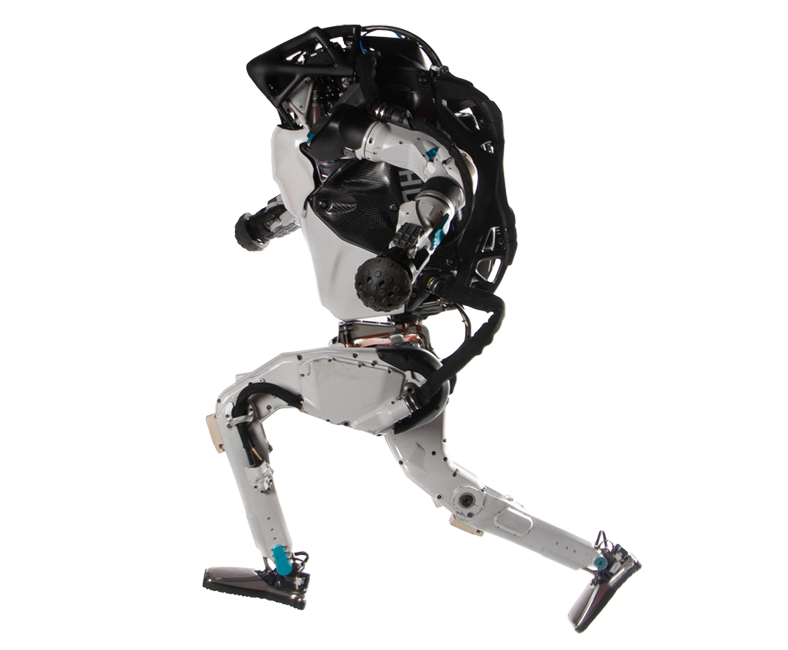
\includegraphics[width=\linewidth]{\picPath/LegRobots/atlas.png}
    \caption{ Двуногий робот Atlas компании Boston dynamics}
  \end{subfigure}
  \begin{subfigure}[b]{0.4\linewidth}
    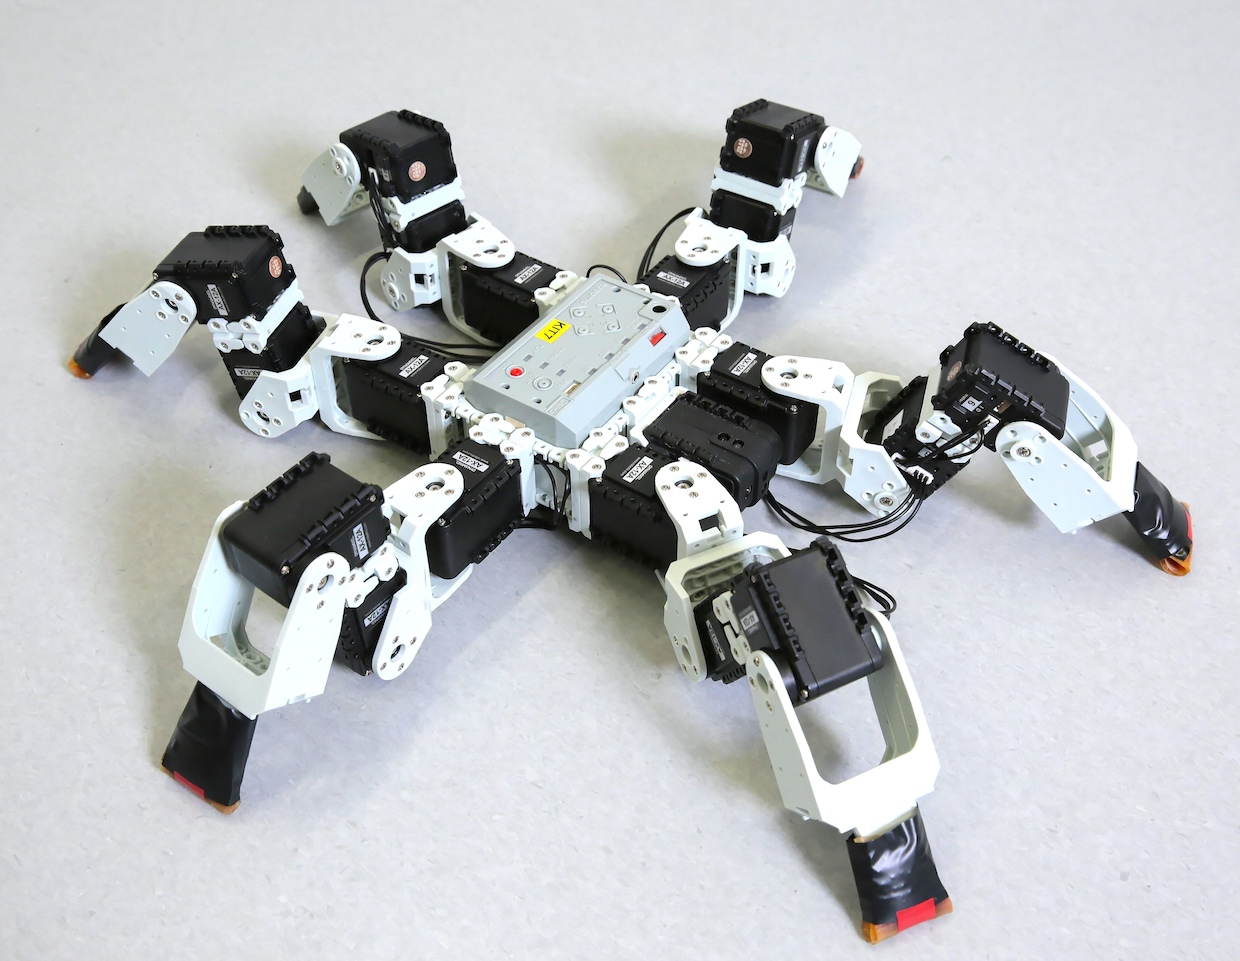
\includegraphics[width=\linewidth]{\picPath/LegRobots/sixLegRobot.jpeg}
    \caption{ Шестиногий робот, результат работы швейцарских исследователей\cite{SixLegsRobots}}
  \end{subfigure}
  \caption{ Современные роботы, использующие ноги для передвижения}
  \label{Figure:LegRobots}
\end{figure}

Основная характеристика роботов, использующих ноги, $-$ последовательность пятен контакта ног робота с поверхностью. Так как для движения такому роботу нужно всего несколько малых областей контакта, качество поверхности не столь важно для его передвижения.

Роботы, использующие ноги, используются в условиях, когда поверхность движения не является плоской или материал поверхности мягкий. Во время качения по плоской твердой поверхности колесо имеет малую площадь соприкосновения с поверхностью, поэтому при качении колесо испытывает малое количество сопротивления. Неровности и мягкий материал поверхности увеличивает площадь поверхности колеса и уменьшает его эффективность. Для создания условий движения колеса требуется большое количество ограничений. Роботы, использующие ноги для движения, в отличие от колесных, имеют большую площадь соприкосновения с поверхностью, что дает им преимущество в сложных условиях.

Роботы, использующие ноги для движения, способны передвигаться в сложных условиях, когда поверхность не является ровной, имеет подъемы или спуски или состоит из мягкого материала. Это позволяет широко использовать таких роботов в сложной среде. Кроме того, такие роботы способны преодолевать препятствия просто перешагивая их. К недостаткам роботов с ногами можно отнести высокую сложность механизма и сравнительно низкую скорость передвижения.

\section{Роботы, использующие колеса для движения}
Использование колес для передвижения - самый распространенный подход к построению мобильных роботов. Во время проектирования роботов, использующих ноги, много внимания уделяется проблеме их устойчивости, в то время как разработка колесных роботов практически лишена этой части проектирования. Несмотря на то, что для устойчивого положения робота в пространстве необходимо всего два колеса, большинство колесных мобильных роботов используют три и более, что решает проблему устойчивости.

Основная задача, стоящая перед проектировщиками мобильных колесных роботов - маневренность и управляемость модели.

Как было описано выше, всякий мобильный робот может быть или голономным, или неголономным. Для случая колесных роботов это значит, что в любой момент времени робот может передвинуться в любом заданном направлении в плоскости. Так например стандартная конфигурация автомобиля не является голономной, в то время как тележка на роликонесущих колесах, описанная ниже, является.

На текущий момент существует множество типов конфигураций колес:
\begin{itemize}
\item обычное колесо;
\item роликовое колесо;
\item роликонесущее колесо.
\end{itemize}
\subsection{Обыкновенное колесо}
Обыкновенное колесо по своей сути $-$ диск или обод, вращающийся на оси или укреплённый на валу и служащий для приведения механизма в движение \cite{Ozhigov}.

Обычное колесо - самый распространенный тип колес, прародитель всех остальных типов, древнейшее изобретение человечества. Такие колеса повсеместно используются в автомобилях, поездах, самолетах и так далее. 

Для того, чтобы вычислить скорость центра обыкновенного колеса в условиях механики сплошных сред, необходимо знать его угловую скорость $\bs{\omega}$, радиус вектор некоторой точки границы диска $\bs{r}$ и скорость точки касания с поверхностью $\bs{V_{0}}$.

Если считать, что скорость поверхности движения равна нулю, то в случае, если вектор скорости $\bs{V_{0}}$ отличен от нуля, колесо скользит по поверхности. 

Тогда скорость центра колеса $\bs{V_{c}}$ будет равна

\begin{equation}
\bs{V_{c}}
=
\bs{V_{0}}
+
\bs{\omega}
\times
\bs{r}
\label{Equation:wheelSpeed}
\end{equation}

Обычное колесо широко используется и в робототехнике. На рисунке \ref{Figure:myCar} изображен робот-шпион, использующий обыкновенные колеса. 

По причине того, что  колесо способно катить колесную тележку только в направлении, перпендикулярном оси его вращения, построение голономного робота, использующего обыкновенные колеса, затруднительно. Для того, чтобы колесный робот на обычных колесах был способен менять направление движения, необходимо менять угол оси его вращения. Так, например, в стандартной конфигурации автомобиля передние оси вращения колес механически соединены с рулевой рейкой, что позволяет маневрировать машиной во время движения.  
\begin{figure}[H]
\begin{center}
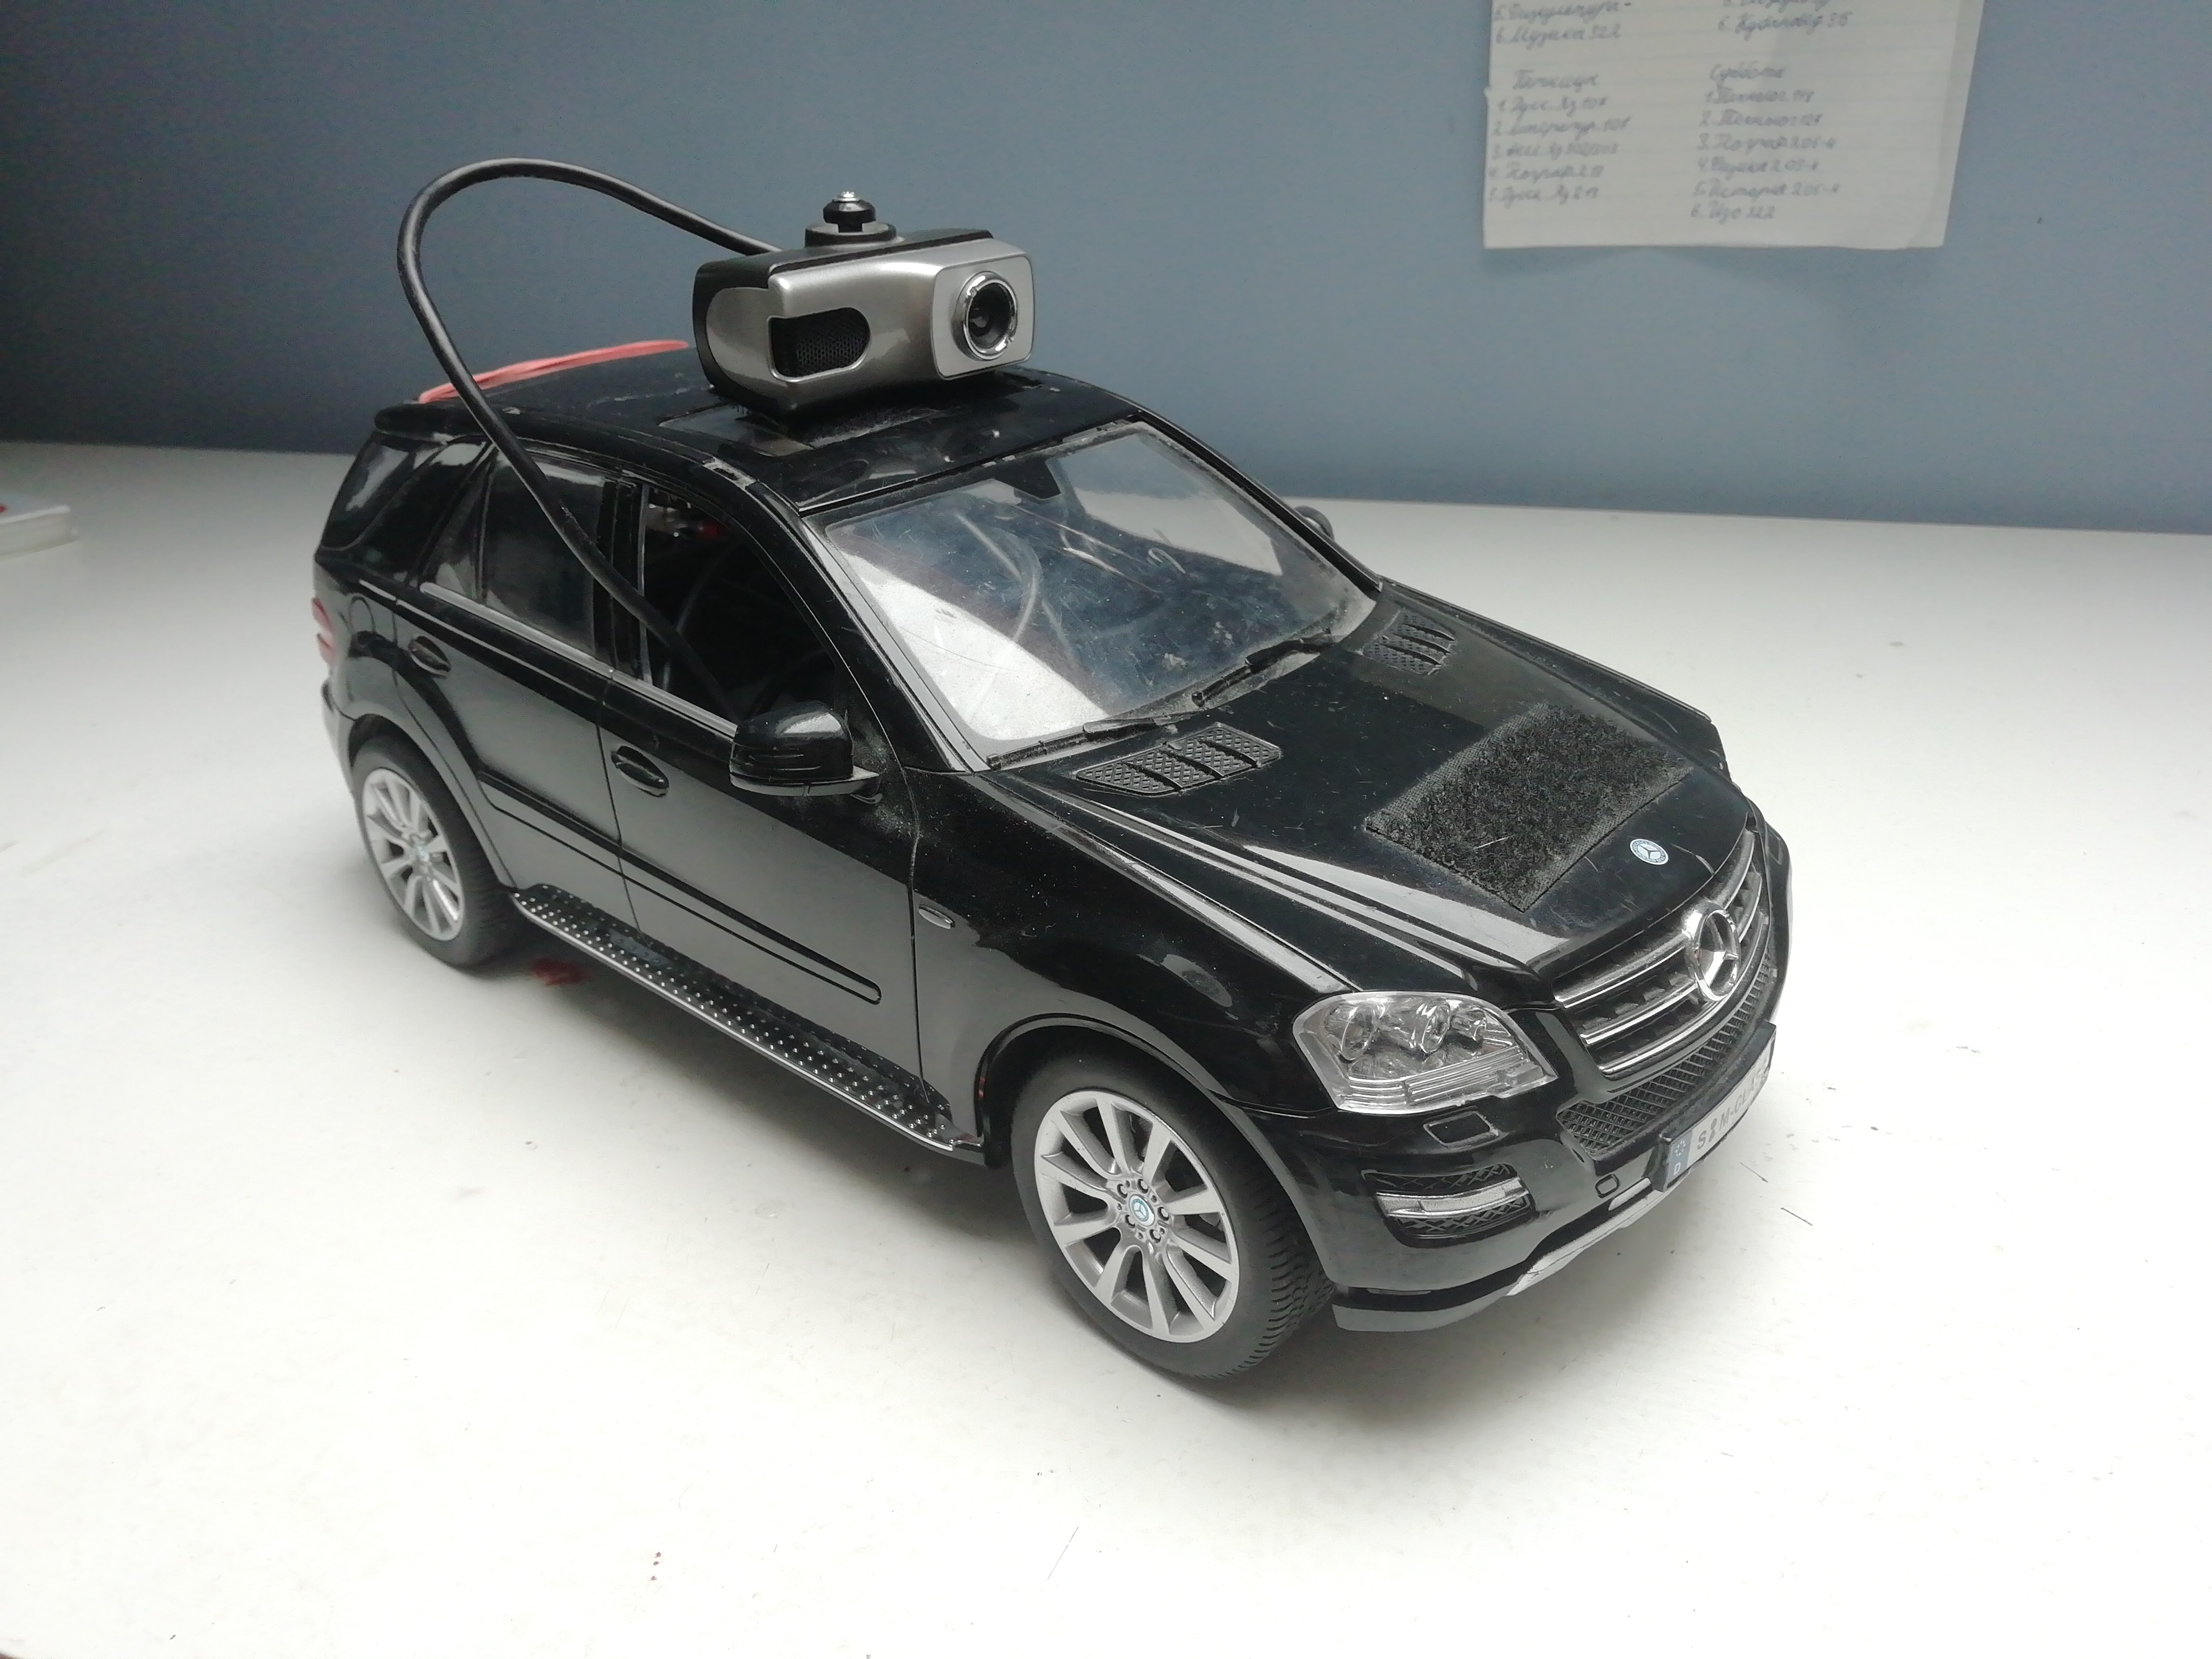
\includegraphics[width=0.5\linewidth]{\picPath/Cars/myCar.jpg}
\end{center}
  \caption{ Робот-шпион, использующий обычные колеса}
  \label{Figure:myCar}
\end{figure}
Главное достоинство обычного колеса - простота конструкции и минимальное трение качения в сравнении другими типами колес \cite{WheelCmp}. К недостаткам относится тот факт, что обычное колесо имеет всего одну степень свободы. \cmmnt{движение обычного колеса возможно только в направлениях, перпендикулярных оси вращения.}
\subsection{Колесо castor wheel}
Castor wheel - распространенный тип колес, повсеместно используемый в каталках, продуктовых тележках, мебели и так далее. У этого типа колес нет определенного русского наименования; будем называть такие колеса роликовыми. Примеры роликовых колес изображены на рисунке \ref{Figure:CastorsWheels}.

Главное отличие роликового колеса от обычного - дополнительная степень свободы. Ось вращения такого колеса может вращается на $360$ градусов. Также, к таким колесам относят закрепленные шарики, способные катиться в любом направлении. 

\begin{figure}[H]
  \centering
  \begin{subfigure}[b]{0.4\linewidth}
   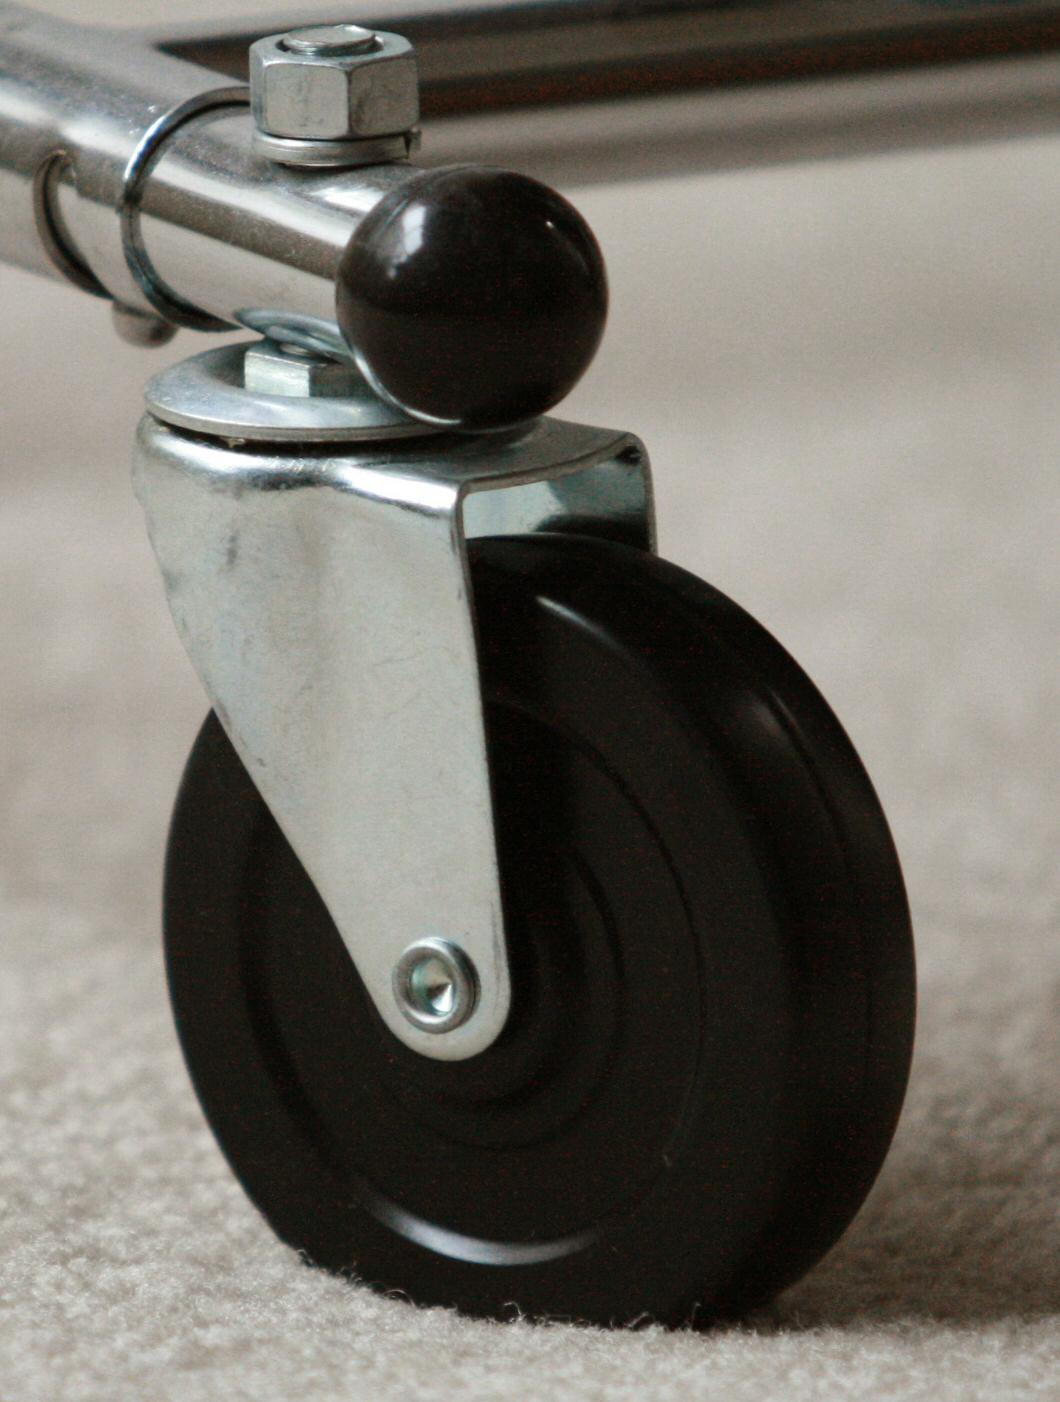
\includegraphics[width=\linewidth]{\picPath/Wheels/castorWheel.jpg}
    \caption{ Роликовое колесо тележки}
  \end{subfigure}
  \begin{subfigure}[b]{0.4\linewidth}
    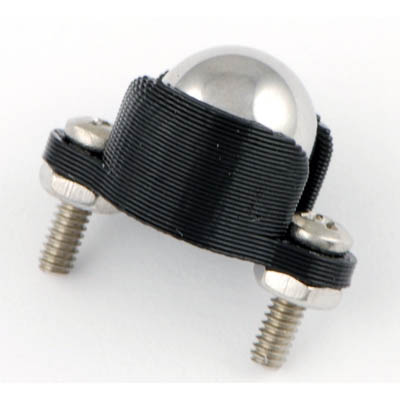
\includegraphics[width=\linewidth]{\picPath/Wheels/simpleBallWeel.jpg}
    \caption{ Шаровое колесо }
  \end{subfigure}
  \caption{ Роликовые колеса}
  \label{Figure:CastorsWheels}
\end{figure}

Благодаря двум степеням свободы роликовые колеса способны катиться в любом направлении. Однако из-за своей конструкции, привести само роликовое колесо в движение затруднительно. Роликовые колеса обычно используется для того, чтобы облегчить движение тяжелых объектов по поверхности, причем объекты приводятся в движения за счет внешних сил. В случае продуктовой тележки, силу для её движения прикладывает покупатель.


В робототехнике роликовые колеса широко используются для увеличения маневренности. Распространенная конфигурация робота, использующего два обычных колеса и одно роликовое, изображена на рисунке \ref{Figure:threeWheelRobot}.
\begin{figure}[H]
\begin{center}
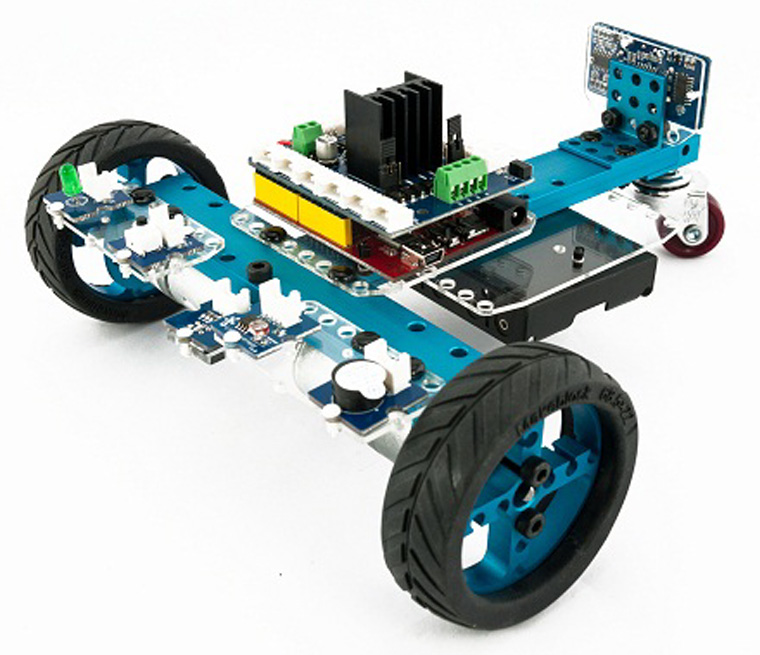
\includegraphics[width=0.4\linewidth]{\picPath/Cars/threeWheels.jpg}
\end{center}
  \caption{ Робот, использующий в своей конфигурации два обычных колеса и одно роликовое}
  \label{Figure:threeWheelRobot}
\end{figure} 
Такая конфигурация позволяет значительно увеличить маневренность робота. Приводя в движение одно из двух колес, тележка вращается на месте, описывая круги вокруг точки касания статичного колеса. Однако такая модель все-еще не является голономной. Движение строго перпендикулярно оси обычный колес все-еще невозможно.

\subsection{Роликонесущее колесо}
Роликонесущее колесо - колесо, имеющее на своем ободе ролики, каждый из которых вращается вокруг собственной оси. Для примера распространенные виды роликонесущих колес изображены на рисунке \ref{Figure:rollerHandedWheels}.
\begin{figure}[H]
  \centering
  \begin{subfigure}[b]{0.4\linewidth}
   \includegraphics[width=\linewidth]{\picPath/Wheels/mecanumWheel.jpg}
    \caption{ колесо Илона }
  \end{subfigure}
  \begin{subfigure}[b]{0.4\linewidth}
    \includegraphics[width=\linewidth]{\picPath/Wheels/omniWheel.jpg}
    \caption{ омни колесо }
  \end{subfigure}
  \caption{ Роликонесущие колеса}
  \label{Figure:rollerHandedWheels}
\end{figure}

Главная характеристика роликонесущего колеса - угол между осью вращения колеса и  осью ролика, касающегося поверхности вращения, $\alpha$. Благодаря вращению роликов, скорость точки касания с поверхностью $\bs{V_{0}}$ из выражения \ref{Equation:wheelSpeed} не равна нулю. Роликонесущее колесо, во время движения, как-бы скользит на установленном на нем ролике в направлении, перпендикулярном оси этого ролика. Это позволяет роботам, использующим такие колеса для передвижения, двигаться в любом заданном направлении. Подробное математическое исследование этого явления описывается в главе \ref{chap:MecanumWheelModel}.

Роликонесущее колесо относительно молодое изобретение. Первое упоминание о нем относится к 1919 году\cite{OmniWheelPatent}, однако в том виде, в котором оно используется сегодня, такое колесо, названное омни колесом, появилось только в	1974 году\cite{OmniWheelPatentModern}. Особенность омни колеса заключается в том, что угол $\alpha = 90^{\circ}$, благодаря чему оно может свободно скользить в любом направлении.

8 апреля 1975 года шведский изобретатель Бенгт Ирланд Илон запатентовал свое изобретение - колесо Илона или, по названию компании, в которой он работал, Mecanum wheel\cite{MecanumWheelPatent}. Инновация заключается в том, что   угол $\alpha$  лежит в пределах $30^{\circ}-60^{\circ}$  градусов, что позволяет устанавливать такие колеса параллельно друг-другу, и при этом не теряя свойство голономности. На рисунке \ref{Figure:holonomicRobots} изображены роботы, использующие для движения роликонесущие колеса типа омни колесо и колесо Илона.


На рисунке \ref{Figure:mecanum_car_simple} изображена возможная конфигурация робота на колесах Илона. Так как угол $\alpha$ непрямой, то устанавливая колеса так, чтобы прямые, проходящие через оси касающихся поверхности роликов, попарно пересекались ($\bs{l_{2}}$,$\bs{l_{3}}$ и $\bs{l_{1}}$,$\bs{l_{4}}$), придем к выводу: вектора скорости точек касания колес с поверхностью не равны нулю и не параллельны. Следовательно, изменяя длину векторов скоростей, возможно задать любое направление движения тележки. В случае омни колеса, колеса не могут находиться параллельно друг-другу: для голономности необходимо, чтобы прямые, проходящие через оси роликов, пересекались. 

\begin{figure}[H]
\centering{
\resizebox{135mm}{!}{\input{mecanum_car_simple.pdf_tex}}
\caption{ модель тележки на четырех колесах Илона}
\label{Figure:mecanum_car_simple}
}
\end{figure}

\begin{figure}[H]
  \centering
  \begin{subfigure}[b]{0.4\linewidth}
   \includegraphics[width=\linewidth]{\picPath/Cars/mecanumWheel.jpg}
    \caption{ мобильный робот, движимый четырмя колесами Илона }
  \end{subfigure}
  \begin{subfigure}[b]{0.4\linewidth}
    \includegraphics[width=\linewidth]{\picPath/Cars/omniWheel.jpg}
    \caption{ мобильный робот, движимый тремя омни колесами }
  \end{subfigure}
  \caption{ Голономные мобильные роботы компании Nexus robot}
  \label{Figure:holonomicRobots}
\end{figure}
Выбор между углом наклона роликов $\alpha$ зависит от поставленной перед мобильным роботом задачей, однако механизм колеса Илона сложнее механизма омни колеса; омни колесо проще в производстве и надежнее. Однако невозможность одновременного расположения омни колес параллельно друг-другу и сохранение голономности делает колесо Илона предпочтительней в случае, когда иные конфигурации невозможны.  

Кроме того, скорость робота при движении параллельно дискам колес, благодаря параллельному расположению, выше: каждое колесо дает положительный вклад в вектор скорости. В то время тележка на омни колесах, ввиду невозможности такой конфигурации, не может двигаться в некотором направлении так, чтобы каждое колесо делало положительный вклад в общее движение.   

Главный недостаток роликонесущих колес - больший вес и высокое сопротивление поверхности качения в сравнении с обычном колесом. Кроме того, устройство роликонесущих колес значительно сложнее устройства обычных, что негативно сказывается на их надежности.
\section{Роботы, использующие гусеницы для движения}
Гусеничный ход $-$ движитель самоходных машин, обеспечивающий повышенную проходимость. Принцип работы гусеничного хода $-$ непрерывное подкладывание гусениц под колёса машины, то есть создание для колёс бесконечного пути, на котором сопротивление движению значительно ниже, чем на мягком грунте\cite{BigSovietEncycl}. Гусеницей, в свою очередь, называется замкнутая сплошная лента или цепь из шарнирно-соединённых звеньев, применяемая в гусеничном ходу . На внутренней поверхности гусеницы имеются впадины или выступы, с которыми взаимодействуют ведущие колёса машины. Внешняя поверхность гусениц снабжена выступами, которые обеспечивают сцепление с грунтом. гусеницы могут быть металлическими, резино-металлическими и резиновыми \cite{BigSovietEncycl}.

Этот тип механизма передвижения распространен среди тяжелой техники и вездеходов. За счет большой площади пятна касания с поверхностью, давление на поверхность движения гораздо меньше, чем в случае других типов колес, благодаря чему транспортные средства не вязнут в рыхлой почве, песке, болотах и так далее. Гусеницы также распространены и среди роботов: такой механизм передвижения позволяет им преодолевать ступени и различные препятствия. 

На практике самая распространенная конфигурация гусеничной машины $-$ два гусеничных хода, расположенных параллельно друг-другу. Пример такой конфигурации изображен на рисунке \ref{Figure:NasaGrover}. Степень свободы гусеничного хода равна единице, однако самоходные гусеничные машины достаточно манёвренные и  способны делать разворот на месте, направляя пару гусеничных ходов в противоположных направлениях с равной скоростью.

\begin{figure}[H]
\begin{center}
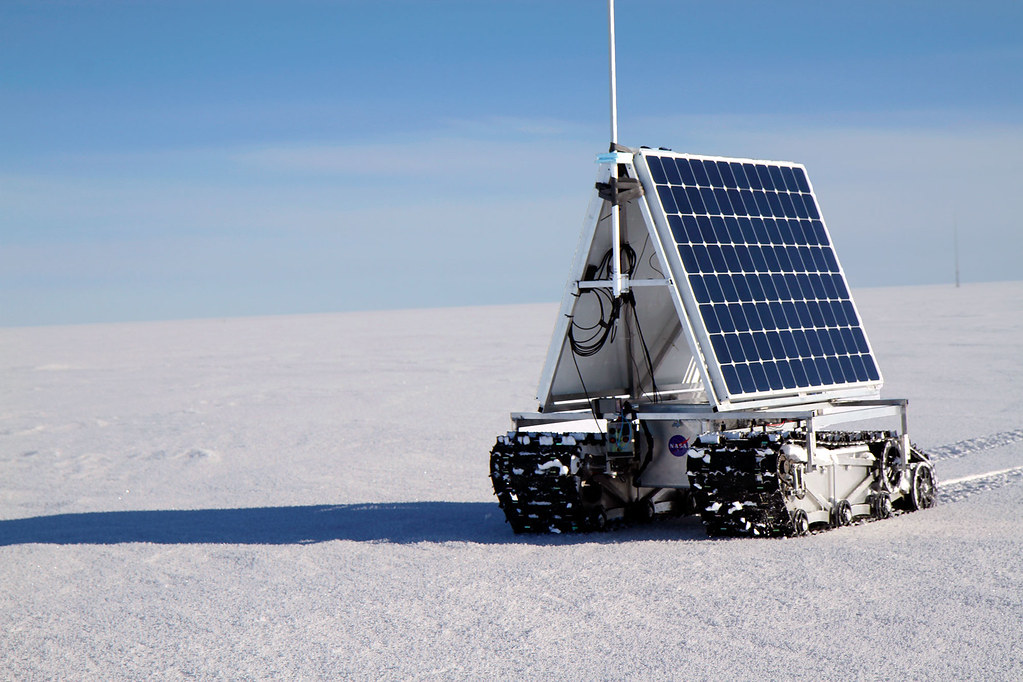
\includegraphics[width=0.5\linewidth]{\picPath/Cars/NasaGrover.jpg}
\end{center}
  \caption{  Гусеничный робот Nasa grover, разработанный для использования в условиях ледяной пустыни }
  \label{Figure:NasaGrover}
\end{figure}

Главный недостаток гусеничных роботов $-$ большая вариация возможных позиций робота после выполнения маневров. Маневрируя, гусеничный робот устанавливает скорость одного из гусеничных ходов отличной от другой, заставляя медленную гусеницу скользить по поверхности. В зависимости от типа поверхности и её состояния, положение робота после маневра может сильно варьироваться \cite{Siegwart}, поэтому точное определение положения гусеничного робота затруднительно. Этот факт затрудняет построение автономного гусеничного робота. Кроме того, большая площадь пятна касания дает большее сопротивление качению, что замедляет робота. Большое количество элементов, содержащееся в гусеничном ходу, подвержено износу и имеет меньший запас прочности, чем обычное колесо. 
\iffalse
Гусеничный ход - компромисс в пользу проходимости робота по пересеченной местности. Несмотря на все недостатки, гусеничные роботы широко в качестве боевых \cite{SaperJournal}.
\fi
\chapter{Кинематическая модель робота с N всенаправленными колесами}  
\label{chap:KinematicOmniWheelModel} 
Описание движения робота требует моделирования его поведения. Простейшая модель движения робота в пространстве - кинематическая. Эта модель описывает движения исключительно через зависимость координат от времени. То есть в кинематической модели рассматривается движение тела, но не рассматриваются причины, его создающие.

Рассматривается движение тележки с $N$ всенаправленными колесами ($N > 3$) по гладкой двумерной поверхности без учета действующих сил, причем плоскости колес тележки вертикальны и неподвижны относительно платформы тележки. В рамках модели всенаправленные колеса способны скользить в любом направлении с пренебрежимо малой силой трения. В рамках модели задается глобальная система координат, связанная с поверхностью $\{o,\boldsymbol{x},\bs{y},\bs{z}\}$ и локальная,  инерциальная относительно глобальной, жестко связанная с тележкой $\{c,\bs{x_{l}},\bs{y_{l}},\bs{z_{l}}\}$, причем плоскость $\bs{x_{l}}\bs{y_{l}}$  параллельна плоскости $\bs{x}\bs{y}$ . Не теряя общности начало локальных координат полагается в точке центра масс тележки. Положение тележки определяется вектором координат $(x,y,\varphi)$
где $x,y$ - координаты на плоскости, и $\varphi$ -  угол между осью $\bs{ox}$ и $\bs{cx_{l}}$. Скорость тележки определяется вектором $(\dot{x},\dot{y},\omega)$ где $\omega = \dot{\varphi}$ - угловая скорость тележки. 

$\{c_{i},\bs{x_{w,i}},\bs{y_{w,i}},\bs{z_{w,i}}\}$ - обозначение локальной системы координат $i$ - го колеса, изображенное на рисунке \ref{fig:omni_wheel_coords}, где $c_{i}$ - ось вращения, $\bs{x_{w,i}}$  - ось, направленная из $c_{i}$  в сторону точки касания с поверхностью, $\bs{y_{w,i}}$ - ось, параллельная поверхности качения, направленная вправо, $\bs{z_{w,i}} = \bs{x_{w,i}} \times \bs{y_{w,i}}$.  

Для примера на рисунке \ref{fig:kinematic_model} схематически изображается кинематическая модель робота с тремя всенаправленными колесами.


\begin{figure}[H]
\centering{
\resizebox{40mm}{!}{\input{omni_wheel_coords.pdf_tex}}
\caption{ координатные оси $i$ - го колеса.}
\label{fig:omni_wheel_coords}
}
\end{figure}

\begin{figure}[H]
\centering{
\resizebox{140mm}{!}{\input{kinematic_model_pic.pdf_tex}}
\caption{ кинематическая модель тележки с тремя всенаправленными колесами.}
\label{fig:kinematic_model}
}
\end{figure}

Вектор скорости $i$- го колеса обозначается как  $\bs{v_{i}}$, $i = \overline{1,N}$. Он направлен по касательной к диску $i$ - го колеса $\bs{y_{w,i}}$. Его разложение на поступательную и  вращательную составляющие имеет вид:
\begin{equation}
\bs{v_{i}}
=
\bs{v_{i,tr}}
+
\bs{v_{i,rot}}
\end{equation}

Обозначения: $\alpha_{i}$ - угол между $\bs{y_{w,i}}$ и осью $\bs{y_{l}}$. Векторы $\bs{v_{i}}$ и $\bs{y_{w,i}}$ сонаправленны, и поэтому $\bs{v_{i}}$ составляет с вектором  $\bs{y_{l}}$ угол $\alpha_{i}$, что иллюстрируется на рисунке \ref{fig:kinematic_model}.



Рассматривается вектор поступательной скорости тележки $\bs{v_{tr}}=[\dot{x},\dot{y},0]$. Для того, чтобы тележка имела скорость $\bs{v_{tr}}$, величина вектора скорости $i$ - го колеса должна быть равна проекции $\bs{v_{tr}}$ на направление $\bs{y_{w,i}}$. Вектор поступательной скорости $i$ - го колеса составляет с осью $\bs{y}$  угол $\varphi + \alpha_{i}$, что иллюстрируется на рисунке \ref{fig:projection}. Тогда $\bs{v_{tr,i}}$ представляется в виде
\begin{equation}
\label{eq:v_rt_i_global}
\bs{v_{tr,i}} 
=
[
-sin(\varphi +\alpha_{i})
\dot{x}
+
cos(\varphi +\alpha_{i})
\dot{y}
]
\bs{y_{w,i}}
\end{equation} 



\begin{figure}[H]
\centering{
\resizebox{70mm}{!}{\input{projection.pdf_tex}}
\caption{ проекция вектора поступательной скорости на направление движения $i$ - го колеса}
\label{fig:projection}
}
\end{figure} 

 Вводятся обозначения: $\bs{R_{i}}$ - радиус вектор оси $i$-го колеса от оси вращения  (точки центра масс) длинны $R_{i}$. Для того, чтобы заставить тележку вращаться вокруг оси вращения $C\bs{z_{l}}$ с угловой скоростью $\omega$, необходимо задать вектор скоростей каждого колеса перпендикулярно $\bs{R_{i}}$. При этом длинна вектора должна составлять $R_{i}\omega$ \cite{Saveliev}.
Таким образом скорости вращательного движения $i$ - го задается следующим уравнением
\begin{equation}
\bs{v_{rot,i}}
=
\bs{R_{i}}
\times
\omega
\bs{z}
\end{equation}

\begin{figure}[H]
\centering{
\resizebox{90mm}{!}{\input{mecanum_wheel_projection3.pdf_tex}}
\caption{ проекция вектора вращательной скорости  $i$ - го колеса на глобальную систему координат}
\label{fig:mecanum_wheel_projection3}
}
\end{figure}

 Вводятся обозначения: $\gamma_{i}$ - угол между осью $\bs{y}$ и  $\bs{R_{i}}$. Тогда результатом проекции $\bs{v_{rot,i}}$   на  $\bs{xy}$, что иллюстрируется на рисунке \ref{fig:mecanum_wheel_projection3} является уравнение 
\begin{equation}
\bs{v_{rot,i}}
=
R_{i}
\omega
[
-cos(\gamma_{i})
\bs{x}
-
sin(\gamma_{i})
\bs{y}
\end{equation}

Результатом проекции $\bs{v_{rot,i}}$ на направление $\bs{y_{w,i}}$, аналогично уравнению \ref{eq:v_rt_i_global}, является
\begin{center}
$
\bs{v_{rot,i}}
=
R_{i}
\omega
[
sin(\varphi + \alpha_{i})
cos(\gamma_{i})
-
cos(\varphi+\alpha_{i})
sin(\gamma_{i})
]
\bs{y_{w,i}}
$
\end{center}
\begin{equation}
\bs{v_{rot,i}}
=
R_{i}
\omega
sin(\varphi+\alpha_{i}-\gamma_{i})
\bs{y_{w,i}}
\end{equation}
Угол $\theta_{i} = \gamma_{i} -\varphi = const$ есть угол между $\bs{R_{i}}$ и $\bs{y_{l}}$, следовательно коэффициент вектора угловой скорости не зависит от $\varphi$ в общем случае. Очевидно $\alpha_{i} - \theta_{i}$ - угол между $\bs{y_{w,i}}$ и $\bs{R_{i}}$. Если касательная диска $i$ - го колеса $y_{w,i}$  перпендикулярна $R_{i}$, то $\alpha_{i} - \theta_{i} = \frac{\pi}{2}, \bs{v_{rot,i}} = R_{i}\omega$. 
\iffalse
 Кроме того, справедливо 
\begin{gather}
\dot{x}
=
v_{x}\bs{x}
\\
\dot{y}
=
v_{y}\bs{y}
\\
\dot{\varphi}
=
\omega\bs{z}
\end{gather}
Где  $v_{x}$, $v_{x}$, $\omega$ - величина скорости по направлению $\bs{x}$ и $\bs{y}$ соответственно, $\omega$ - величина угловой скорости.
\fi 

Таким образом вектор скорости $i$ - го колеса записывается в виде:
\begin{equation}
\label{eq:local_v_global}
\bs{v_{i}}
=
[
-sin(\varphi +\alpha_{i})\dot{x}
+cos(\varphi +\alpha_{i})\dot{y}
+
R_{i}
\omega
sin(\alpha_{i} - \theta_{i})
]
\bs{y_{w,i}}
\end{equation}



Вводятся обозначения: $\omega_{i}$ - искомая угловая скорость $i$ - го колеса.
Результатом соотношения вектора скорости $i$ - го колеса с его угловой скоростью является
\begin{equation}
\label{eq:local_v_local}
\bs{v_{i}}
=
\bs{r_{i}}
\times
\omega_{i}
\bs{z_{w,i}}
\end{equation}

Где $\bs{r_{i}}$  - вектор, имеющий координаты $[-r_{i},0,0]$ в системе координат $i$-го колеса тележки, $r_{i}$ - радиус $i$ -го колеса тележки, $\omega_{i}$ - угловая скорость этого колеса.
Результатом вычисления векторного произведения в \ref{eq:local_v_local} является 
\begin{equation}
\label{eq:local_v_local_res}
\bs{v_{i}}
=
\bs{r_{i}}
\times
\omega_{i}
\bs{z_{w,i}}
=
\omega_{i}
r_{i}
\bs{y_{w,i}}
\end{equation}
% получим зависимость величины угловой скорости колеса от тройки  $(\dot{x},\dot{y},\omega)$

Таким образом, результатом выражения  $w_{i}$ из \ref{eq:local_v_local_res} и подстановки $\bs{v_{i}}$ из \ref{eq:local_v_global} является уравнение:
\begin{equation}
\omega_{i}
=
\frac{1}{r_{i}}
(
-sin(\varphi +\alpha_{i})\dot{x}
+cos(\varphi +\alpha_{i})\dot{y}
+
R_{i}
\omega
sin(\alpha_{i} - \theta_{i})
)
\end{equation}

или в матричной форме 

\begin{equation}
\label{eq:kinematic_omniwheel_res}
\begin{bmatrix}
\omega_{1} \\
\omega_{2} \\
...\\
\omega_{N}
\end{bmatrix}
=
\begin{bmatrix}
-\frac{1}{r_{1}}sin(\varphi +\alpha_{1}) &
\frac{1}{r_{1}}cos(\varphi +\alpha_{1}) &
\frac{1}{r_{1}}R_{1}sin(\alpha_{1} - \theta_{1})
\\
-\frac{1}{r_{2}}sin(\varphi +\alpha_{2}) &
\frac{1}{r_{2}}cos(\varphi +\alpha_{2}) &
\frac{1}{r_{2}}R_{2}sin(\alpha_{2} - \theta_{2})
\\
... & ... & ...
\\
-\frac{1}{r_{N}}sin(\varphi +\alpha_{N}) &
\frac{1}{r_{N}}cos(\varphi +\alpha_{N}) &
\frac{1}{r_{N}}R_{N}sin(\alpha_{N} - \theta_{N})
\end{bmatrix}
\begin{bmatrix}
\dot{x} \\
\dot{y} \\
\omega
\end{bmatrix}
\end{equation}

Таким образом, координаты траектории пути $(x,y,\varphi)$ однозначно определяют величину угловой скорость каждого колеса. Для нахождения угловой скорости каждого колеса необходимо вычислить $(\dot{x},\dot{y},\omega)$ и подставить в формулу \ref{eq:kinematic_omniwheel_res}.

\iffalse
Кроме того, переходя к локальным координатам

\begin{equation}
\begin{bmatrix}
\dot{x} \\
\dot{y} \\
\omega
\end{bmatrix}
=
\begin{bmatrix}
cos(\varphi) & 0 & 0 \\
0 & cos(\varphi) & 0 \\
0 & 0 & 1
\end{bmatrix}
\begin{bmatrix}
\dot{x_{l}} \\
\dot{y_{l}} \\
\omega
\end{bmatrix}
\end{equation}

Получаем уравнение движения тележки в локальной системе координат
\begin{equation}
\begin{bmatrix}
\dot{\phi_{1}} \\
\dot{\phi_{2}} \\
...\\
\dot{\phi_{N}}
\end{bmatrix}
=
\begin{bmatrix}
-\frac{1}{r_{1}}sin(\varphi +\alpha_{1}) &
\frac{1}{r_{1}}cos(\varphi +\alpha_{1}) &
\frac{1}{r_{1}}R_{1}sin(\alpha_{1} - \theta_{1})
\\
-\frac{1}{r_{2}}sin(\varphi +\alpha_{2}) &
\frac{1}{r_{2}}cos(\varphi +\alpha_{2}) &
\frac{1}{r_{2}}R_{2}sin(\alpha_{2} - \theta_{2})
\\
... & ... & ...
\\
-\frac{1}{r_{N}}sin(\varphi +\alpha_{N}) &
\frac{1}{r_{N}}cos(\varphi +\alpha_{N}) &
\frac{1}{r_{N}}R_{N}sin(\alpha_{N} - \theta_{N})
\end{bmatrix}
\begin{bmatrix}
cos(\varphi) & 0 & 0 \\
0 & cos(\varphi) & 0 \\
0 & 0 & 1
\end{bmatrix}
\begin{bmatrix}
\dot{x_{l}} \\
\dot{y_{l}} \\
\omega
\end{bmatrix}
\end{equation}

где $\dot{x_{l}}$,$\dot{y_{l}}$ - величина скорости по направлению $X_{l}$ и  $Y_{l}$ соответственно.
\fi

\chapter{Динамическая модель робота с N всенаправленными колесами}
Динамическая модель, в отличие от кинематической, рассматривает движение твердых тел с учетом сил, приводящих это тело в движение.Тележка приводится в движения за счет крутящего момента $T$. 
 
В рамках этой главы рассматривается движение тележки с $N$ всенаправленными колесами ($N > 3$) по негладкой двумерной поверхности с учетом действующих сил. В описании модели используются те же обозначения, что и в кинематической модели за исключением того, что вместо векторов скорости рассматриваются векторы сил $\bs{f_{i}}$. Сила $\bs{f_{i}}$ приложена к верхней точке $i$ - го колеса в направлении качения. Для примера на рисунке \ref{fig:dynamic_model} схематически изображена динамическая модель робота с тремя всенаправленными колесами. Равнодействующая всех сил, действующих на тележку $\bs{F}$ имеет вид:
\begin{equation}
\bs{F}
=
F_{x}\bs{x}
+
F_{y}\bs{y}
+
M_{t}\bs{z}
\end{equation} 

Сила как мера воздействия на тело характеризует поступательное движение модели, в то время как момент сил $M_{t}\bs{z}$ характеризует вращательное движение. Равнодействующую всех сил можно разложить на поступательную и вращательную составляющие, аналогично кинематической модели, следующим образом:
\begin{equation}
F
=
\begin{bmatrix}
F_{X} \\
F_{Y} \\
M_{t}
\end{bmatrix}
=
\begin{bmatrix}
M & 0 & 0 \\
0 & M & 0 \\
0 & 0 & J_{r}
\end{bmatrix}
\cdot
\begin{bmatrix}
\ddot{x}\\
\ddot{y} \\
\dot{\omega}
\end{bmatrix}
=
B \cdot \ddot{u}
\end{equation}

Где $M$ - масса тележки, $J_{r}$ - её момент инерции. 

\begin{figure}[H]
\centering{
\resizebox{140mm}{!}{\input{dynamic_model_pic.pdf_tex}}
\caption{ динамическая модель тележки с тремя всенаправленными колесами}
\label{fig:dynamic_model}
}
\end{figure}
Момент инерции тележки можно считать приближенно равным моменту инерции однородного цилиндра радиуса $R=max_{i}(R_{i})$ 
\begin{equation}
J_{r}
=
\frac{1}{2}
MR^{2}
\end{equation}


Кроме того, вектор $\bs{F}$ можно представить в  виде:
\begin{equation}
\bs{F}
=
\sum_{i=1}^{N}\bs{f_{i}}
\end{equation}
где $\bs{f_{i}}$ - вектор силы, приложенной верхней точке $i$ - го колеса. Имеет направление $\bs{y_{w,i}}$, величину $f_{i}$ и составляет с осью $\bs{y}$ угол $\varphi + \alpha_{i}$.  
Тогда, результатом разложения $\bs{F}$ по компонентам и проекции вектора $\bs{f_{i}}$ на координатные оси является

\begin{equation}
\bs{F_{X}}
=
-
\bs{x}
\sum_{i=1}^{N}f_{i} sin(\varphi +\alpha_{i})
\end{equation}
\begin{equation}
\bs{F_{Y}}
=
\bs{y}
\sum_{i=1}^{N}f_{i} cos(\varphi +\alpha_{i})
\end{equation}
\begin{equation}
\label{eq:rot_force}
\bs{M_{t}}
=
\sum_{i=1}^{N}\bs{f_{i}}\times\bs{R_{i}}
=
\bs{z}
\sum_{i=1}^{N}f_{i}R_{i}sin(\alpha_{i} - \theta_{i})
\end{equation}



Величины компонент вектора сил связываются следующим образом:
\begin{equation}
\begin{bmatrix}
F_{X} \\
F_{Y} \\
M_{t}
\end{bmatrix}
=
\begin{bmatrix}
-sin(\varphi + \alpha_{1}) &
-sin(\varphi + \alpha_{2}) &
...              &
-sin(\varphi + \alpha_{N}) \\
cos(\varphi + \alpha_{1}) &
cos(\varphi + \alpha_{2}) &
...              &
cos(\varphi + \alpha_{N}) \\ 
R_{1}sin(\alpha_{1} - \theta_{1}) &
R_{2}sin(\alpha_{2} - \theta_{2}) &
 ... &
R_{N}sin(\alpha_{N} - \theta_{N})
\end{bmatrix}
\begin{bmatrix}
f_{1} \\
f_{2} \\
...   \\
f_{n}
\end{bmatrix}
=
Af
\end{equation}

Результатом является уравнение
\begin{equation}
F = A\bs{f}
\label{eq:f}
\end{equation}

Результатом разрешения уравнение \ref{eq:f} относительно $f$ является
\begin{equation}
\bs{f}
=
A^{-1}
\cdot
F
=
A^{-1}
\cdot
B 
\cdot
\bs{
\ddot{u}
}
\end{equation}

Зная, что вращающий момент колеса равен силе, приложенной в его верхней точке на его радиус и обозначая 
\begin{equation}
\bs{r} 
=
\begin{bmatrix}
r_{1} \\
r_{2} \\
... \\
r_{N}
\end{bmatrix}
\end{equation}
возможно описать зависимость координат пути $(x,y,\varphi)$ от крутящих моментов каждого колеса:
\begin{equation}
\label{eq:dynamic_w_friction}
\begin{bmatrix}
T_{1} \\
T_{2} \\
... \\
T_{N}
\end{bmatrix}
=
\bs{r}
\bs{
f}
^{T}
=
\overline{r}
(
A^{-1}
\cdot
B 
\cdot
\bs{\ddot{u}}
)^{T}
\end{equation}

В свою очередь величину момента сил каждого колеса можно выразить через его угловое ускорение:

\begin{equation}
T_{i}
=
J_{w,i}\dot{\omega_{i}}
\end{equation}

Где $J_{w,i}$ - момент инерции $i$-го колеса,$\dot{\omega_{i}}$ - угловое ускорение $i$ - го колеса.

Учтем силу трения качения модели по некоторой поверхности, предполагая равномерное распределение веса на каждое колесо. Известно, что сила трения качения противоположна по направлению силе, приводящей колесо в действие и для $i$-го колеса может быть вычислена по формуле:
\begin{equation}
f_{t_{i}}
=
\frac{Mg\eta}{Nr_{i}}
\end{equation}

Где $Mg$ - сила реакции опоры, равная силе тяжести робота, $\eta$ - коэффициент трения качения, зависящий от характеристик поверхности. $\eta = 0$ в случае, когда трения между колесом и поверхностью не происходит и $\eta = \infty$ когда трение поверхности непреодолимо сильно.  
Сила трения качения направлена в противоположную сторону от направления движения колеса. Поэтому для того, чтобы её компенсировать, необходимо увеличить силу, приложенную в верхней точке колеса на величину силы трения.
\begin{equation}
\tilde{f_{i}}
=
f_{i}
+
f_{t_{i}}
\end{equation}

Вводятся обозначения
\begin{equation}
\bs{\tilde{f}}
=
\bs{f}
+
\begin{bmatrix}
f_{t_{1}} \\
f_{t_{2}} \\
... \\
f_{t_{N}}
\end{bmatrix}
=
\bs{f}
+
\frac{Mg\eta}{N}
\cdot
\begin{bmatrix}
\frac{1}{r_{1}} \\
\frac{1}{r_{2}} \\
...       \\
\frac{1}{r_{N}}
\end{bmatrix}
\end{equation}

Тогда заменяя в формуле \ref{eq:dynamic_w_friction} $f$ на $\tilde{f}$, определяется зависимость момента сил каждого колеса от координат пути, учитывающая силу трения:
\begin{equation}
\label{eq:res_dinamic_omniwheel}
\begin{bmatrix}
T_{1} \\
T_{2} \\
... \\
T_{N}
\end{bmatrix}
=
\bs{r}
(
A^{-1}
\cdot
B 
\cdot
\bs{
\ddot{u}
}
+
\frac{Mg\eta}{N}
\cdot
\begin{bmatrix}
\frac{1}{r_{1}} \\
\frac{1}{r_{2}} \\
...       \\
\frac{1}{r_{N}}
\end{bmatrix}
)^{T}
\end{equation} 

Таким образом уравнение \ref{eq:res_dinamic_omniwheel} определяет динамическая модель тележки, учитывающую её массу и силу трения качения. Зная координаты пути $\bs{u} = (x,y,\varphi)$ и вычисляя ускорение для каждой координаты $\bs{\ddot{u}} = (\ddot{x},\ddot{y},\dot{\omega})$, из уравнения \ref{eq:res_dinamic_omniwheel} определяются соответствующие заданному пути моменты сил каждого колеса.

\iffalse
В работе ref более детально рассматривается динамическая модель тележки на N роликонесущих колесах.  Модель тележки строится исходя из предположения о том, что модель роликонесущего колеса — твердый диск, скорость наинизшей точки которого перпендикулярна направлению оси ролика в этой точке. Кроме того, рассмотрен критерий управляемости такой модели, из которого следует ряд ограничений на его конструкцию. Например если сумма угла оси ролика и угла поворота колеса всех роликонесущих колес равна, то такая модель не может двигаться по произвольной трактории. Если же эти углы у двух колес совпадают, то пару колес можно принять за одно виртуальное колесо с радиус вектором $r_{ij} = r_{i} - r_{j}$ в локальной системе координат и моментом $T_{ij} = T_{i} + T_{j}$.
\fi
\chapter{Кинематическая модель роликонесущего колеса} 
\label{chap:MecanumWheelModel}
Для нероликонесущегого колеса, которое вращается по поверхности без скольжения, мгновенная скорость низшей точки касания равна нулю \cite{MecanumWheel}. На практике соприкасающиеся тела из-за физических ограничений всегда соприкасаются множеством точек, называемым пятном контакта. В качестве иллюстрации можно привести гусеничную тележку, двигающуюся по поверхности без просткальзываний. Пятно касания гусеницы достаточно большое чтобы заметить, что в определенное мгновение оно не двигается относительно поверхности. При достаточно низкой скорости тележки можно заметить, что некоторая подобласть пятна касания гусеницы не двигается относительно поверхности некоторый промежуток времени. 

Особенность роликонесущих колес заключается в том, что мговенная точка касания имеет ненулевую скорость относительно поверхности качения, так как укрепленные на колесе ролики под силой тяжести тележки вращаются относительно своей оси. \cmmnt{В случае всенаправленного колеса, оси роликов которого параллельны плоскости диска колеса, проскальзывания не происходит, что упрощает процесс построения математической модели}

 Простейшей неголономной моделью роликонесущего колеса является плоский диск, для которого скорость точки соприкосновения с несущей поверхностью направленная вдоль прямой, составляющий постоянный угол с плоскостью колеса.

\begin{figure}[H]
\centering{
\resizebox{160mm}{!}{\input{mecanum_disk.pdf_tex}}
\caption{модель роликонесущего колеса: вид сбоку}
\label{fig:mecanum_disk_side}
}
\end{figure}

\begin{figure}[H]
\centering{
\resizebox{130mm}{!}{\input{mecanum_wheel_top.pdf_tex}}
\caption{ модель роликонесущего колеса: вид сверху}
\label{fig:mecanum_disk_top}
}
\end{figure}

 В качестве модели роликонесущего колеса рассматривается диск радиуса $R$ с центром в точке $C$, причем плоскости колес тележки вертикальны и неподвижны относительно платформы тележки\cite{MecanumWheel}. Обозначения: $\bs{l}$ - единичный вектор оси вращения ролика, $\bs{\tau}$ - касательная к плоскости диска, $\delta = \widehat{\bs{l} \bs{\tau}}$. Тогда уравнение связи имеет вид:
\begin{equation}
(
\bs{v_{M}}
,
\bs{l}
)
=
0
\end{equation}
где $M$ - точка касания, $\bs{v_{M}}$ - скорость точки касания. Вектор $\bs{v_{M}}$ определяется следующим образом:
\begin{equation}
\bs{v_{M}}
=
\bs{v_{C}}
+
\bs{\omega}
\times
\bs{CM}
\end{equation}
где
$\bs{v_{C}}$ -   
скорость центра колеса, $\bs{\omega}$ - вектор угловой скорость колеса.
Обозначения: $\{O,\bs{e_{x}},\bs{e_{y}},\bs{e_{z}}\}$ - глобальная инерциальная система координат, $\{C,\bs{E_{x}},\bs{E_{y}},\bs{E_{z}}\}$ - система координат, жестко связанная с диском. Плоскость $\{C,\bs{E_{x}},\bs{E_{y}}\}$ параллельна плоскости поверхности.  $\varphi$ - угол поворота диска вокруг перпендикулярной плоскости диска оси, проходящей через точку $C$ против часовой стрелки, $\psi = \widehat{\bs{\tau} \bs{e_{x}}}$. Обозначения иллюстрируются на рисунках \ref{fig:mecanum_disk_side} и \ref{fig:mecanum_disk_top}. Тогда вектора $\bs{\omega}$ и $\bs{CM}$ можно представить в виде:
\begin{equation}
\bs{\omega}
=
\dot{\varphi}
\bs{E_{y}}
+
\dot{\psi}
\bs{E_{z}}
\end{equation}
\begin{equation}
\bs{CM}
=
-R
\bs{E_{z}}
\end{equation}

Отсюда справедливо
\begin{equation}
\bs{\omega}
\times
\bs{CM}
=
-R\dot{\varphi}
\bs{E_{x}}
\end{equation} 

Обозначая за $x_{C}$ $y_{C}$ координаты точки $C$ в глобальных координатах, проектируя вектор скорости точки $C$ на локальную систему координат, что иллюстрируется на рисунке \ref{fig:mecanum_wheel_projection}, верно уравнение:
\begin{equation}
\label{eq:velocity_c_projection}
\bs{v_{C}}
=
(
\dot{x_{C}}
cos\psi
+
\dot{y_{C}}
sin\psi
)
\bs{E_{x}}
+
(
-\dot{x_{C}}
sin\psi
+
\dot{y_{C}}
cos\psi
)
\bs{E_{y}}
\end{equation}

\begin{figure}[H]
\centering{
\resizebox{100mm}{!}{\input{mecanum_wheel_projection.pdf_tex}}
\caption{ иллюстрация проектирования вектора скорости на локальную систему координат}
\label{fig:mecanum_wheel_projection}
}
\end{figure}

Проецируя единичный вектор $l$ на локальную систему координат: 
\begin{equation}
\bs{l}
=
cos\delta
\bs{E_{x}}
+
sin\delta
\bs{E_{y}}
\end{equation}

определяем уравнение связи в виде
\begin{flushleft}
$
(
\bs{v_{m}}
,
\bs{l}
)
=
(
\bs{v_{c}}
+
\bs{\omega}
\times
\bs{CM}
,
\bs{l}
)
=
$

$
(
(
\dot{x_{C}}
cos\psi
+
\dot{y_{C}}
sin\psi
-R\dot{\varphi}
)
\bs{E_{x}}
+
(
-\dot{x_{C}}
sin\psi
+
\dot{y_{C}}
cos\psi
)
\bs{E_{y}}
,
cos\delta
\bs{E_{x}}
+
sin\delta
\bs{E_{y}}
)
=
$

$
(
\dot{x_{C}}
cos\psi
+
\dot{y_{C}}
sin\psi
-R\dot{\varphi}
)
cos\delta
+
(
-\dot{x_{C}}
sin\psi
+
\dot{y_{C}}
cos\psi
)
sin\delta
=
0
$
\end{flushleft}
\begin{equation}
\label{eq:mecanum_final}
\dot{x_{C}}
cos(\psi+\delta)
+
\dot{y_{C}}
sin(\psi+\delta)
=
R\dot{\varphi}
cos\delta
\end{equation}

Уравнение \ref{eq:mecanum_final} связывает между собой тройку координат $(x_{C},y_{C},\psi)$ с угловой скоростью колеса $\varphi$. В работе \cite{MecanumWheelCartDynamic} изучена динамика тележки с $N$ роликонесущими колесами и сформулирован критерий управляемости:
если $N \geq 3$, хотя бы одна пара векторов  $\bs{l_{i}}, \bs{l_{j}}$ $i,j=\overline{1,N}$, которые соответствуют осям роликов, не параллельна и точки контакта колес не лежат на одной прямой, то для любой траектории всегда возможно найти такие управляющие моменты (то есть функции $\varphi_{i}(t)$), что тележка, управляемая этими моментами, переместится по заданной траектории.

\chapter{Кинематическая модель тележки на четырех роликонесущих колесах}
В рамках данной главы рассматривается кинематическую модель тележки на четырех роликонесущих колесах, проиллюстрированная на рисунке  \ref{fig:mecanum_car}. Обозначения: $C$ - точка вращения тележки, $\{O,\bs{e_{x}},\bs{e_{y}},\bs{e_{z}}\}$ - глобальная инерциальная система координат, $\{C,\bs{E_{x}},\bs{E_{y}},\bs{E_{z}}\}$ - система координат, жестко связанная с тележкой. Плоскость $\{C,\bs{E_{x}},\bs{E_{y}}\}$ параллельна плоскости поверхности.  $r_{i}$ - радиус $i$ -го колеса, $\delta_{i}$ - угол между касательной к плоскости колеса $\bs{p_{i}}$ и осью ролика $\bs{l_{i}}$\cmmnt{, $\delta_{i} = \widehat{p_{i} l_{i}}$ }, $\psi$ - угол между осью $\bs{e_{x}}$ и $\bs{E_{x}}$\cmmnt{, $\psi$ = $\widehat{e_{x}E{x}}$}, $\alpha_{i}$ - угол между осью $\bs{E_{x}}$ и радиус вектором $\bs{R_{i}}$ длинны $R_{i}$, направленным из точки $C$ в точку касания с поверхностью $i$-го колеса $C_{i}$\cmmnt{,$\alpha_{i} = \widehat{E_{x}\overrightarrow{C C_{i}}}$}, $i=\overline{1,4}$. 

\begin{figure}[H]
\centering{
\resizebox{170mm}{!}{\input{mecanum_car.pdf_tex}}
\caption{ модель тележки на четырех роликонесущих колесах }
\label{fig:mecanum_car}
}
\end{figure}

Рассматривается вектор скорости центра $i$-го колеса $\bs{v_{c,i}}$. Результатом его разложения на поступательную и вращательную составляющие является:
\begin{equation}
\label{eq:mec_wheel_v_decomp}
\bs{v_{c,i}}
=
\bs{v_{tr,i}}
+
\bs{v_{rot,i}}
\end{equation}

Вектор поступательной скорости $\bs{v_{tr,i}}$ имеет координаты $[\dot{x},\dot{y},0]$. Уравнение связи с угловой скоростью $i$ - го колеса $\varphi_{i}$, основываясь на уравнении \ref{eq:mecanum_final} имеет вид:
\begin{equation}
\dot{x}
cos(\psi+\delta)
+
\dot{y}
sin(\psi+\delta)
=
r_{i}\dot{\varphi_{i}}
cos\delta_{i}
\end{equation}
Где $[\dot{x},\dot{y},0]$ - координаты вектора поступательной скорости тележки.
 
Для того, чтобы заставить тележку вращаться вокруг оси вращения $C\bs{E_{z}}$, необходимо задать вектор скоростей каждого колеса перпендикулярно радиус вектору $\bs{R_{i}}$. При этом длинна вектора должна составлять $R_{i}$\cite{Saveliev}. Расположение векторов иллюстрируется на  рисунке \ref{fig:mecanum_car_rot}.

\begin{figure}[H]
\centering{
\resizebox{150mm}{!}{\input{mecanum_car_rot.pdf_tex}}
\caption{ вращение тележки на четырех роликонесущих колесах вокруг оси вращения}
\label{fig:mecanum_car_rot}
}
\end{figure}

Рассматривается вектор вращательной скорости $i$ - го колеса $\bs{v_{rot,i}}$. Результатом его проекции на оси $\bs{E_{x}}$ $\bs{E_{y}}$, как показано на рисунке \ref{fig:mecanum_wheel_projection1}, является
\begin{equation}
\bs{v_{rot,i}}
=
R_{i}
\dot{\psi}
sin(\alpha_{i})
\bs{E_{x}}
-
R_{i}
\dot{\psi}
cos(\alpha_{i})
\bs{E_{y}}
\end{equation}

\begin{figure}[H]
\centering{
\resizebox{80mm}{!}{\input{mecanum_wheel_projection1.pdf_tex}}
\caption{ проекция вектора вращательной скорости на локальную систему координат}
\label{fig:mecanum_wheel_projection1}
}
\end{figure}

Результатом проекции вектора $\bs{v_{rot,i}}$ на оси $\bs{e_{x}}$ $\bs{e_{y}}$, как изображается на рисунке \ref{fig:mecanum_wheel_projection2} , является

$
\bs{v_{rot,i}}
=
R_{i}
\dot{\psi}
sin\alpha_{i}
(
cos\psi \bs{e_{x}}
+
sin\psi \bs{e_{y}}
)
-
R_{i}
\dot{\psi}
cos\alpha_{i}
(
-sin\psi \bs{e_{x}}
+
cos\psi \bs{e_{y}}
)
$
\begin{equation}
\label{eq:v_rot_global}
\bs{v_{rot,i}}
=
R_{i}
\dot{\psi}
sin(\alpha_{i} + \psi)
\bs{e_{x}}
-
R_{i}
\dot{\psi}
cos(\alpha_{i} + \psi)
\bs{e_{y}}
\end{equation}

\begin{figure}[H]
\centering{
\resizebox{80mm}{!}{\input{mecanum_wheel_projection2.pdf_tex}}
\caption{ проекция вектора вращательной скорости на глобальную систему координат}
\label{fig:mecanum_wheel_projection2}
}
\end{figure}

Тогда результатом подстановки \ref{eq:v_rot_global} в уравнение связи \ref{eq:mecanum_final} является выражение:

$
R_{i}
\dot{\psi}
sin(\alpha_{i} + \psi)
cos(\psi + \delta_{i})
-
R_{i}
\dot{\psi}
cos(\alpha_{i} + \psi)
sin(\psi + \delta_{i})
=
r_{i}\dot{\varphi_{i}}
cos\delta_{i}
$
\begin{equation}
R_{i}
\dot{\psi}
sin(\alpha_{i} - \delta_{i})
=
r_{i}
\dot{\varphi}
cos\delta_{i}
\end{equation}

Тогда уравнение связи для $\bs{v_{c,i}}$, исходя из \ref{eq:mec_wheel_v_decomp}, принимает вид
\begin{equation}
\label{eq:res_mecanum_wheel_car}
\dot{x}
cos(\psi+\delta_{i})
+
\dot{y}
sin(\psi+\delta_{i})
+
R_{i}
\dot{\psi}
sin(\alpha_{i}-\delta_{i})
=
r_{i}\dot{\varphi_{i}}
cos\delta_{i}
\end{equation}
Результатом выражения $\dot{\varphi_{i}}$ из \ref{eq:mec_wheel_v_decomp} является
\begin{equation}
\label{eq:res_mecanum_wheel_ang_v}
\dot{\varphi_{i}}
=
\frac{
  \dot{x}
  cos(\psi+\delta_{i})
  +
  \dot{y}
  sin(\psi+\delta_{i})
  +
  R_{i}
  \dot{\psi}
  sin(\alpha_{i}-\delta_{i})
}
{
  r_{i}cos\delta_{i}
}
\end{equation}

При чисто поступательном ($\dot{\psi_{i}} = 0$) или чисто вращательном ($\dot{x}=\dot{y}=0$) движении связь \ref{eq:res_mecanum_wheel_ang_v} является голономной, то есть угловое ускорение каждого колеса не зависит от предыдущих движений робота. В противном случае, для вычисления \ref{eq:res_mecanum_wheel_ang_v} необходимо учитывать текущий угол поворота следующим образом:
\begin{equation}
\psi
=
\int\limits_{t_{0}}^{t_{cur}} \psi(t) dt
\end{equation}
Где $t_{0}$, $t_{cur}$ - начальный и текущий момент времени соответственно.

Таким образом представляется зависимость величины угловой скорости от координат пути. Для того, чтобы найти угловую скорость $i$ - го колеса, $i=\overline{1,4}$, соответствующую заданному пути $(x,y,\psi)$, необходимо вычислить $(\dot{x},\dot{y},\dot{\psi})$ и подставить в уравнение \ref{eq:res_mecanum_wheel_ang_v}.

\chapter{Технолигии моделирования робототехнических систем}
\section{Фреймворк для программирования робототехнических систем ROS }
ROS (Robot Operating System  -  операционная система для роботов) -  фреймворк с открытым исходным кодом, нацеленный на реализацию программного обеспечения для роботизированных систем\cite{ros.org}.  ROS включает в себя коллекцию инструментов, библиотек и соглашений, нацеленных на упрощение разработки сложных роботизированных систем разных конфигураций.
 
Другими словами ROS -  уровень абстракции над аппаратными средствами робототехнических систем. Однако несмотря на то, что в названии присутствует связка операционная система, ROS операционной системой не является. Для функционирования ROS необходима операционная система в привычном смысле; ROS поддерживает множество linux дистрибутивов, а также windows и android.  В некокоторых источниках такую модель абстракции называют мета-операционной системой.

После установки, ROS предоставляет следующие функциональные возможности \cite{RosBookTurtle}: 
\begin{itemize}
\item Распределенный процесс: робототехническая система представляется как множество связанных друг с другом узлов, каждый из которых работает независимо от остальных;
\item Использование пакетов: несколько программных компонентов или узлов, непосредственно связанных друг с другом можно объединить в пакет, который легко интегрируется в другую робототехническую систему;
\item API: поставляемые вместе с системой ROS библиотеки позволяют управлять внутренними процессами системы посредством распространенных языков программирования: python, C++, lisp и другими.
\end{itemize}

В открытом доступе доступно множество пакетов, которые реализуют управление кинематикой, методы компьютерного зрения совместно с библиотекой openCV, измерение параметров окружения с помощью физических датчиков и сенсоров, построение карт окружения робота, планирование маршрута в двумерном и трехмерном пространстве и другие.

Система ROS нацелена на ускорение развития робототехники в целом, понижая порог входа в область построения роботов. Используя доступные пакеты и существующие системы, разработка роботизированных систем значительно ускоряется. 

Архитектура системы ROS делится на следующие уровни:
\begin{itemize}
\item уровень файловой системы;
\item уровень графа вычислений системы;
\item уровень глобального распространения пакетов.
\end{itemize}

\subsection{Уровень файловой системы}
На этом уровне архитектуры системы ROS описывается элементы, хранящиеся в памяти операционной системы
\begin{itemize}
\item пакет;
\item мета-пакет;
\item пакетный манифест;
\item репозиторий;
\item определение типов сообщений
\item определение сервисных типов 
\end{itemize}

Здесь и далее термины определяются в контексте системы ROS.

Пакет $-$ главная единица организации программного обеспечения. Пакет может содержать узлы, связанные библиотеки, файлы данных, конфигурацию и любую другую информацию, необходимую для описания пакета.  Пакет - единица компиляции или сборки программного обеспечения робота, содержащая в себе конфигурацию, необходимую для компиляции. 

Мета-пакет $-$ специализированный пакет, включающий в себя исключительно информацию для правильной компиляции пакета инструментом catkin. Catkin - официальная система сборки пакетов ROS, являющаяся по сути множеством макросов распространенной системы сборки CMake.

Пакетный манифест $-$ файл формата XML, имеющий фиксированное имя - package.xml и хранящий такие метаданные пакета, как его наименование, список разработчиков, сторонние зависимости и другую мета-информацию. Структура файла строго определена в специализированном документе.

Репозиторий $-$ коллекция пакетов, совместимых с одной из версий системы  ROS.

Определение типов сообщений $-$ файлы, хранящиеся обычно в подпапке /msg и имеющие расширение  .msg . Эти файлы хранят в себе описание определенных разработчиком типов сообщений. Такое сообщение состоит из одного или нескольких объектов стандартного типа std_msgs или производных типов. 

Определение сервисных типов $-$ файлы, хранящиеся обычно в подпапке /srv, определяющие структуру запросов и ответов определенных разработчиком сервисов ROS.
\subsection{Уровень графа вычислений системы}

Графом вычислений в контексте системы ROS называется сеть связанных друг с другом узлов, работающих независимо друг от друга и общающихся посредством передачи сообщений. 
На рисунке \ref{Figure:gazeboGraph} можно видеть пример такого графа, изображенного с помощью инструмента rqt_graph.


\begin{figure}[H]
\begin{center}
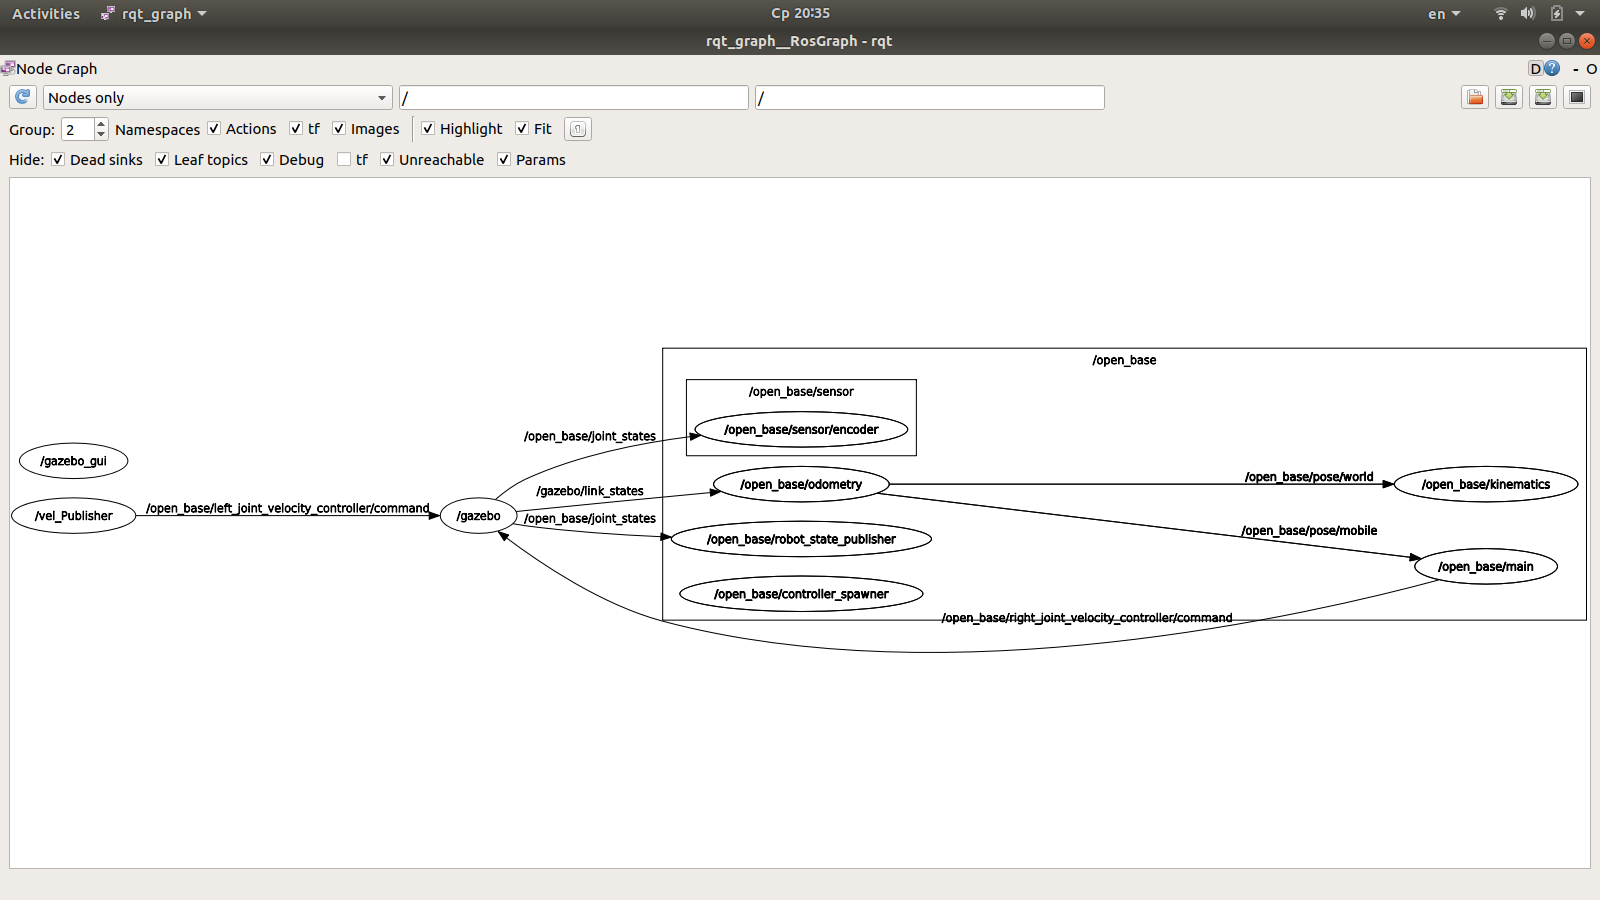
\includegraphics[width=0.95\linewidth]{\picPath/Gazebo/compGraph.png}
\end{center}
  \caption{ граф вычислений во время тестирования роботизированной тележки }
  \label{Figure:gazeboGraph}
\end{figure}


Граф вычислений состоит из следующих элементов:

\begin{itemize}
\item узел (node);
\item главный сервис управления - мастер (master);
\item сообщение (message);
\item тема (topic);
\item сервис (service);
\item рюкзак (bag).
\end{itemize}

Узел $-$  процесс, производящий некоторые вычисления, играющий роль подписчика и издателя в топологии вычислительного графа. 

Мастер, или главный сервис управления $-$ программа, регистрирующая узлы и сервисы в графе вычислений и отвечающая за связь узлов между собой. Для связи элементов графа мастер использует tcp/ip протокол, что позволяет связывать узлы графа по сети.   

Сообщение $-$ структура данных, передаваемая между узлами. Состоит из стандартных std_msgs или производных типов данных.

Тема $-$  промежуточное звено между узлами. Коммуникация между узлами вычислительного графа подчиняется шаблону проектирования издатель-подписчик. В контексте ROS, каждый узел является как издателем, так и подписчиком. Для того, чтобы связать два узла, необходимо определить тему, через который будет происходить коммуникация. Узел-издатель публикует сообщение по адресу темы, в то время как узел-подписчик подписывается на эту тему и получает уведомление каждый раз, когда по её адресу передается сообщение. Такой подход к построению топологии позволяет увеличить независимость вычислительных узлов.

Сервис $-$ процесс, производящий некоторые вычисления, подчиняющийся шаблону проектирования запрос-ответ. Используется в тех случаях, когда необходимо установить двустороннюю связь между процессами. 

Рюкзак $-$ формат хранения последовательно передаваемых данных. Позволяет сохранять и воспроизводить последовательности сообщений во времени.

\subsection{Формат описания робототехнических систем  URDF}
\label{chapt:URDF}
Архитектура ROS описывает способы ведения вычислений связанных с робототехнической системой, однако не позволяет описать таковую. Для описания роботов в системе ROS используется формат URDF.

URDF (Universal Robotic Description Format) $-$ формат описания робототехнических систем в трехмерном пространстве, основанный на XML. Документ представляет из себя XML файл с предопределенным набором тегов. Робот представляется как совокупность звеньев (link) и сочленений (joint). Кроме того, в URDF файле возможно описание сенсоров и других вспомогательных параметров. 

Корневым элементом модели является тег <robot> с атрибутом name, в который вкладываются теги звеньев <link> и сочленений <joint>.

Звено (link) описывает твердое тело с инерцией, визуальными особенностями и физическими ограничениями. Звено содержит в себе следующие элементы, описывающие:

\begin{itemize}
\item момент инерции <inertial>
\item внешний вид твердого тела <visual>
\item границы коллизии <collision>
\end{itemize}

Описание момента инерции, кроме непосредственно тензора инерции, включает в себя такие параметры, как относительный сдвиг, поворот инерциальных координат и массу.

Внешний вид определяется цветом, текстурой и формой объекта. В качестве формы могут использовать как стандартные типы (параллелепипед, цилиндр, сфера), так и трехмерные модели. 

Границы коллизии описывают границы твердого тела. Используется для обнаружения пересечений между собой двух или более объектов. Разделение внешнего вида от границ коллизии позволяет значительно ускорить вычисления в случае сложной визуальной модели, вычисления коллизии с которой не является принципиальным элементом симуляции системы. 

Описывая робототехническую систему, состоящую из нескольких звеньев, необходимо задать информации о их сочленении. В описании URDF используются следующие типы сочленений:
\begin{itemize}
\item фиксированное сочленение (fixed);
\item шарнирное сочленение (revolute) задает ось и границы вращения звеньев относительно друг друга;
\item непрерывное сочленение  (continious) является шарнирным соединением без ограничений на угол поворота
\item призматическое сочленение (prismatic) позволяет одному звену двигаться относительно другого вдоль некоторой прямой;
\item планарное сочленение (palnar) позволяет одному звену двигаться относительно другого в некоторой плоскости;
\item плавающее сочленение (floating) позволяет одному звену двигаться относительно другого в трех измерениях.
\end{itemize} 

Каждый тег сочленения содержит в себе ссылку на опорное звено, звено-родитель <parent>, и, соответственно, движимое звено, звено-наследник <child>.  В зависимости от типа тег сочленения включает в себя описание оси и границ вращения, ограничения на скорость вращения, силу трения между сочленением и другие параметры\cite{ros.org}. 

\section{Среда моделирование робототехнических систем Gazebo}
\label{chap:Gazebo}
Gazebo $-$ среда моделирования робототехнических систем в трехмерном пространстве с открытым исходным кодом. Имеет поддержу нескольких пакетов моделирования физических процессов, таких как ODE, Bullet, DART и других. Gazebo позволяет симулировать реальное окружение и сценарии среды, для которой разрабатывается робототехническая система. Кроме того, среда моделирования Gazebo позволяет симулировать реалистичные сигналы для виртуальных датчиков, таких как стерео камеры, системы лазерного измерения расстояния между объектами LIDAR и других сенсоров.
На рисунке \ref{Figure:gazeboEx} изображается процесс моделирования трехколесной тележки. 

\begin{figure}[H]
\begin{center}
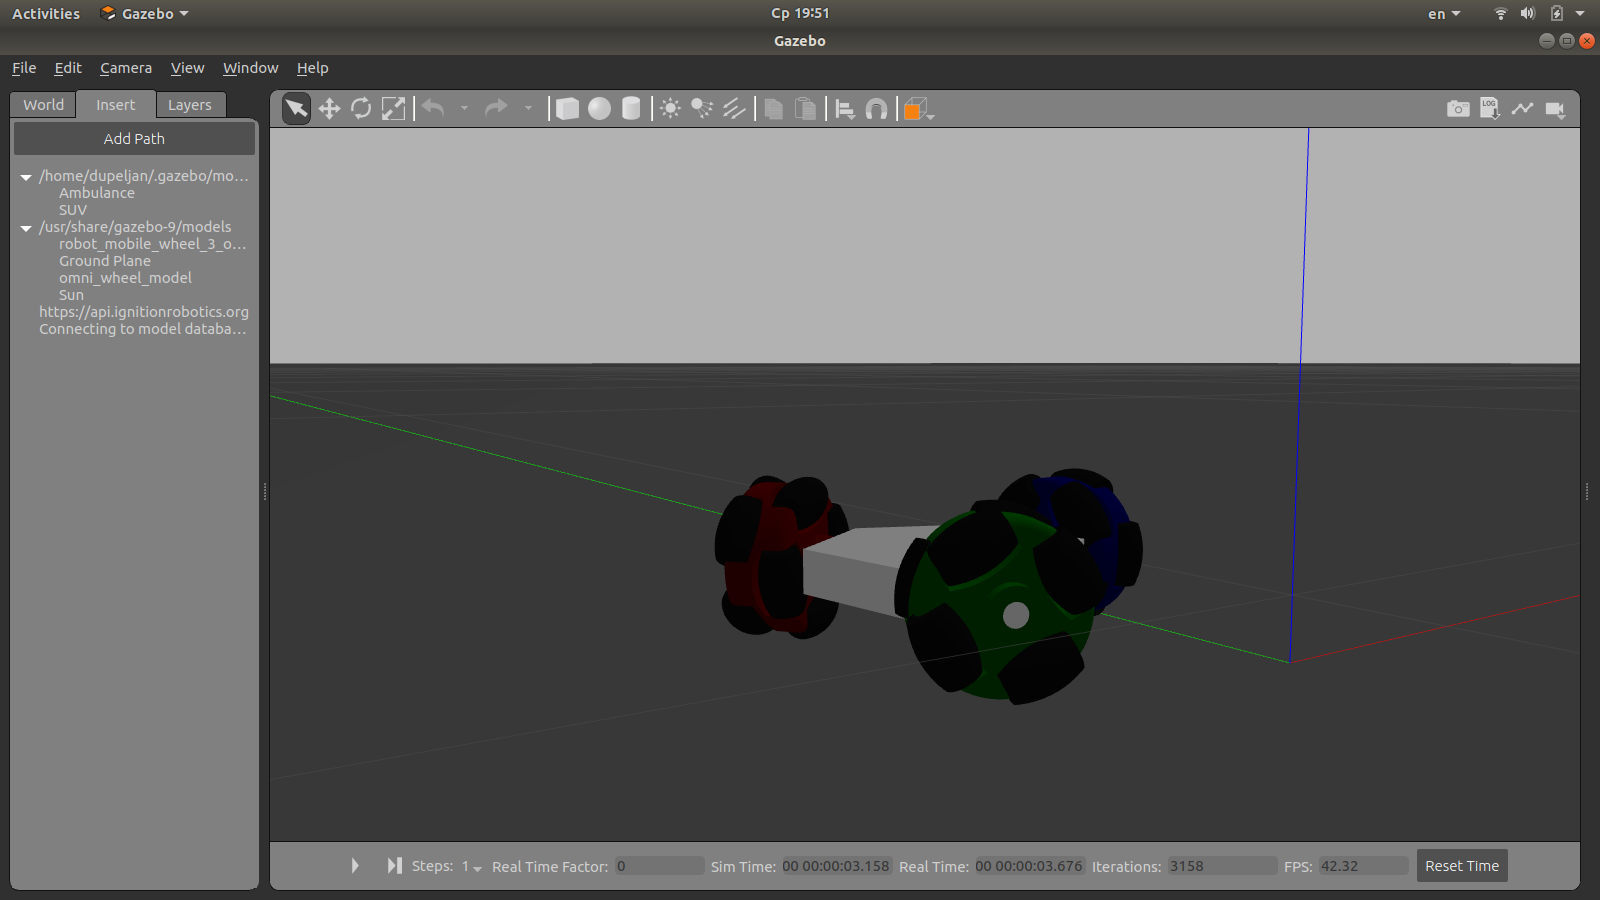
\includegraphics[width=1\linewidth]{\picPath/Gazebo/cart.png}
\end{center}
  \caption{ Симуляция трехколесной тележки в среде симуляции Gazebo}
  \label{Figure:gazeboEx}
\end{figure}

Среда Gazebo повсеместно используется в соревнованиях, работе и исследованиях таких компаний, как Nasa, Toyotа, DARPA и других компаниях \cite{gazebosim.org}. 

Для моделирование робототехнических систем Gazebo предоставляет формат SDF, альтернативный формату URDF. Формат SDF во многом схож с URDF: оба  являются диалектом языка XML и описывают модель робота с помощью  совокупности звеньев и сочленений. Однако, кроме этого, формат SDF позволяет изменять параметры симуляции и содержит описание сенсоров и плагинов управления роботом. С помощью SDF файлов описывается расположение и конфигурация объектов, в том числе других SDF или URDF моделей, на сцене. 

Для того, чтобы смоделировать сцену, среде моделирования Gazebo необходимо передать стартовый SDF файл, содержащий описание сцены, которую необходимо смоделировать. Роботизированная система, попадая в симуляцию, подчиняется кофигурации окружающей среды, заданной в стартовом SDF файле. По умолчанию на систему действует сила тяжести, сила трения, и другие силы. 

Управление симуляцией возможно с помощью плагинов Gazebo. Плагин представляет из себя скомпилированную библиотеку, присоединяющуюся к объекту симуляции через SDF файл. Имеется множество встроенных плагинов управления кинематикой, камерой и другими сенсорами. Кроме того, с помощью Gazebo API - набора библиотек взаимодействия с программой Gazebo, возможно описать собственный плагин управления симуляцией. 

Плагины Gazebo делятся на следующие категории:
\begin{itemize}
\item плагин окружения (word);
\item плагин модели (model);
\item плагин системы (system);
\item плагин визуальных параметров (visual);
\item плагин графического интерфейча (gui);
\item плагин сенсора (sensor).
\end{itemize}

Каждый тип плагина управляется отдельным компонентом Gazebo. Например, плагин модели присоединяется к конкретной модели и позволяет управляет ею. Плагин окружения подключается к среде моделирования, а плагин сенсора - к определенному сенсору. 

Функциональность плагина зависит от его типа. Плагин окружения используется для управления свойствами симуляции, такими как физический характеристики симуляции, окружающее освещение и так далее. Плагин модели используется для управления сочленениями модели. Плагин сенсора используется для получения информации о сенсоре и управления его характеристиками.

\section{Системы автоматического управления. ПИД регуляторы}
Как известно из механики твердых тел для того, чтобы в инерциальной системе исчисления заставить тело двигаться, необходимо приложить к нему силу, придавая тем самым ускорение этому телу. В реальных условиях невозможно придать телу бесконечное ускорение, поэтому тело достигает определённой скорости только через определенный момент времени \cite{Saveliev}. 

Теория систем автоматического управления изучает способы своевременного установления определенного состояния некоторой системы. В частности, в качестве системы можно рассматривать ведущее колесо тележки, а в качестве состояния $-$ определенная скорость вращения этого колеса \cite{pidBook}.

Распространенный способ управления состоянием системы $-$  использование пропорционально-интегрально-дифференцирующего регулятора (ПИД). ПИД регулятор $-$ устройство в управляющем контуре с обратной связью. Его устройство проиллюстрировано  на рисунке \ref{fig:PID}.


\begin{figure}[H]
\centering{
\resizebox{150mm}{!}{\input{PID_en.pdf_tex}}
\caption{ Схема устройства ПИД регулятора }
\label{fig:PID}
}
\end{figure}

На вход ПИД регулятора поступает два сигнала: требуемая величина некоторой характеристики $r(t)$ и реальное значение этой характеристики $y(t)$. В реальных системах сигнал  $y(t)$ снимается с помощью сенсоров или датчиков. В случае ПИД регуляции температуры этот показатель может быть показатель датчика температуры. 

На следующем этапе вычисляется значение ошибки $e(t)$  как 
\begin{equation}
e(t)
=
r(t) - y(t)
\end{equation}

после чего вычисляется величина корректировки $u(t)$ :
\begin{equation}
u(t)
=
K_{p} e(t)
+
K_{i} \int\limits_{0}^{t} e(t) dt
+
K_{d} 
\frac{d e(t)}{dt}
\end{equation} 

Где $K_p$, $K_i$, $K_d$ $-$ характеристики ПИД регулятора, коэффициенты  пропорциональной, интегральной и дифференциальной составляющих соответственно.

Величина $u(t)$ добавляется к управляющему сигналу $r(t)$, корректируя его поведение. 

В случае дискретной функции управления $r(n), n \in N$ величина ошибки и корректировки вычисляется следующим образом:
\begin{equation}
\label{Equation:discretError}
e(n) 
=
r(n)
-
y(n)
\end{equation}
\begin{equation}
u(n)
=
K_p e(n)
+
K_i^{discr} \sum\limits_{k=0}^n e(k)
+
K_d^{disct} (e(n) - e(n-1)) 
\end{equation}

где $K_p$, $K_i^{discr}$, $K_d^{discr}$ $-$ коэффициенты  пропорциональной, интегральной и дифференциальной дискретных составляющих соответственно.

Подбирая коэффициенты элементов ПИД регулятора, можно добиться устойчивой работы системы. Правильная настройка регулятора позволяет достаточно быстро компенсировать  отклонения от требуемого значения некоторых параметров системы, приближая теоретические расчеты  параметров к реальным. 

\chapter{Программная реализация}
\section{ SDF модель }
\label{chap:SDFCartModel}

В качестве моделируемой роботизированной системы в работе используется тележка, приводимая в действие тремя омни-колесами. 
Модель имеет следующие характеристики, проиллюстрированные на рисунке \ref{fig:cartScheme}
\begin{figure}[H]
\centering{
\resizebox{120mm}{!}{\input{cart.pdf_tex}}
\caption{ Схема моделируемой трехколесной тележки }
\label{fig:cartScheme}
}
\end{figure}

Расстояние до центра масс до каждого колеса $R = 0.04$ единицы, радиус колеса $r = 0.01905$ единиц. Угол $\beta$, проиллюстрированный на рисунке \ref{fig:cartScheme} равен $120^{\circ}$, углы $\gamma_i$ между осью $\bs{x}$ и $\bs{v_i}$ равны $150, 270, 30$ градусов соответственно.


\begin{figure}[H]
  \centering
  \begin{subfigure}[b]{0.4\linewidth}
   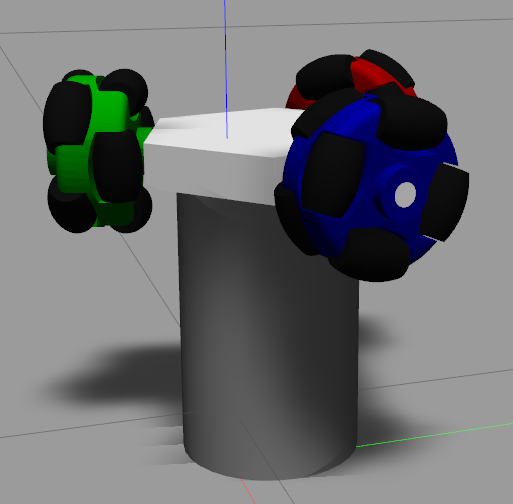
\includegraphics[width=\linewidth]{\picPath/Gazebo/cartOnly.png}
    \caption{ трехколесная тележка }
  \end{subfigure}
  \begin{subfigure}[b]{0.4\linewidth}
    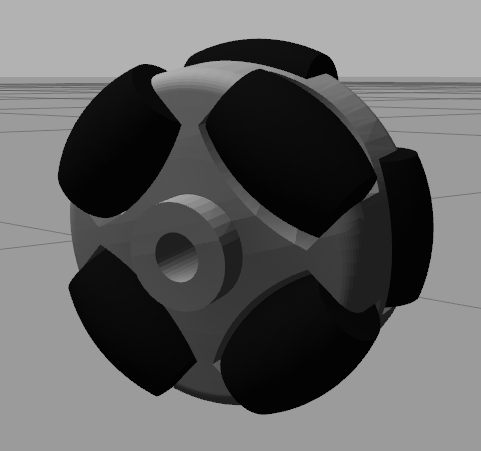
\includegraphics[width=\linewidth]{\picPath/Gazebo/omniWheel.png}
    \caption{ омни-колесо}
  \end{subfigure}
  \caption{ SDF модели в симуляции Gazebo}
  \label{Figure:gazeboModels}
\end{figure}

На рисунке \ref{Figure:gazeboModels} иллюстрируются смоделированные модели: модель омни-колеса и трехколесная тележка, опирающаяся на три таких омни-колеса. Каждое омниколесо меет на своем ободе восемь роликов, каждый из которых вращается вокруг собственной оси. Все соединения имею шарнирный тип revolute, описывающийся в главе \ref{chapt:URDF}.
\section{ Плагин модели Gazebo} 
Для управления моделью тележки в данной работе используется Gazebo API, а именно плагин уровня модели. Плагин позволяет двигать тележку в любом заданном направлении голономно, то есть без вращения вокруг собственной оси. Плагин имеет два режима работы: управление непосредственно с помощью команд, поступающих извне и следование по заданному маршруту. 

После подключения к симуляции, плагин начинает публиковать тему, в которой сообщается положение робота на плоскости. Эта информация используется клиентским приложением, описанным в следующей главе. 
Кроме того, плагин подписывается на тему /"имя робота"/velocity типа VelocityWheels. Описание типа сообщения содержится в файле /msg/VelocityWheels.msg. 

Клиентское приложение, это может быть любой узел, подписавшийся на эту тему, публикует величину скорости в тему  /"имя робота"/velocity. Плагин получает эти сообщения и изменяет скорости колес с помощью функции setTargetVelocity.

Функция  

setTargetVelocity(double left,double right, double back) 

задает скорости каждого колеса. Для устойчивого управления используется четыре ПИД регулятора, реализация которых включается в Gazebo API. Три ПИД регулятора подключены в цепь управления скоростью вращения колес. Gazebo API  позволяет получать реальную скорость вращения колес, что соответсвует дискретной функции $y(n)$ из выражения \ref{Equation:discretError}.  

Требуется, чтобы движения тележки  были голономными. Для этого используется четвертый ПИД регулятор, использующий в качестве $e(t)$ величину отклонения поворота тележки от оси абсцисс  глобальной системы координат.

Для регулирования парамметров ПИД регуляторов используется стандартный пакет динамической настройки параметров dynamic_reconfigure. В функции, вызываемой при загрузке плагина, создается поток чтения запросов о изменении параметров, описанных в файле PIDconf.cfg.  Посредством утилиты  rqt_reconfigure  в поток посылаются запросы на изменение конфигурации, обрабатываемые плагином. 


Сообщение /"имя робота"/velocity имеет поле stop. Передавая по адресу темы скорость, с полем stop = true, плагин переконфигурируется в режим следования по аналитически заданному пути. Плагин отписывается от текущей темы и подписывается на тему /"имя робота"/path типа PathMsg.Описание типа сообщения содержится в файле /msg/PathMsg.msg. 

Далее плагин ожидает первого уведомление по этой теме. Перове сообщение содержит в себе вектор точек $-$ аналитический маршрут. Первый элемент вектора $-$ стартовая точка маршрута, последний элемент $-$ финальная. Тележка из своего текущего местоположения отправляется в начальную точку и после, проходя через все промежуточные точки маршрута, хранящиеся последовательно в полученном векторе, достигает финальной точки и останавливается. По окончании следования аналитическому пути плагин переконфигурируется и заново подписывается на тему  /"имя робота"/velocity.

\section{Алгоритм движения тележки по аналитически заданному пути}
\label{chap:cartMovingAlg}
Для движения в заданном направлении с заданной скоростью используется вывод главы \ref{chap:KinematicOmniWheelModel}. Согласно характеристикам, описанным в главе \ref{chap:SDFCartModel}, уравнение \ref{eq:kinematic_omniwheel_res} принимает вид:

\begin{equation}
\label{eq:realOmniWheelCart}
\begin{bmatrix}
\omega_{1} \\
\omega_{2} \\
\omega_{3}
\end{bmatrix}
=
\frac{1}{r}
\begin{bmatrix}
-sin(\varphi +\alpha_{1}) &
cos(\varphi +\alpha_{1}) &
R
\\
-sin(\varphi +\alpha_{2}) &
cos(\varphi +\alpha_{2}) &
R
\\
-sin(\varphi +\alpha_{3}) &
cos(\varphi +\alpha_{3}) &
R
\end{bmatrix}
\begin{bmatrix}
\dot{x} \\
\dot{y} \\
\omega
\end{bmatrix}
\end{equation}

где углы $\alpha_1$, $\alpha_2$, $\alpha_3$ равны соответственно $150, 270, 30$ градусов.

фиксируя величину линейной скорости тележки $v = const$, и зная текущее и требуемое положение тележки на плоскости $p_0$, $p_1$, при этом  
\begin{equation}
p_i 
= 
\begin{bmatrix}
x_i
\\
y_i
\end{bmatrix} 
\end{equation}

определяются величины скоростей вращения колес тележки из \ref{eq:realOmniWheelCart}; вектор скорости тележки заменяется на следующее выражение:

\begin{equation}
\begin{bmatrix}
\dot{x} \\
\dot{y} \\
\omega
\end{bmatrix}
=
v
\begin{bmatrix}
\frac{x_1 - x_0}{norm} \\
\frac{y_1 - y_0}{norm} \\
0
\end{bmatrix}
=
\bs{v_{desired}}
\end{equation}
\begin{equation}
norm = \sqrt{(x_1 - x_0)^2 + (y_1 -y_0)^2}
\end{equation}

Для того, чтобы тележка преодолела расстояние $r$ единиц  по прямой  со скоростью $v$ единиц в секунду, необходимо поддерживать скорость $v$  в течение $\frac{r}{v}$ секунд. Однако на практике движение тележки из-за физических помех является нелинейным. Зная реальную скорость вращения колес, используя преобразование, обратное \ref{eq:realOmniWheelCart}, определяется реальная скорость тележки:

\begin{equation}
\label{eq:reverseRealOmniWheelCart}
\begin{bmatrix}
\dot{x}_{real} \\
\dot{y}_{real} \\
\omega_{real}
\end{bmatrix}
=
\frac{2r}{3 \sqrt{3} R }
\begin{bmatrix}
-\frac{\sqrt{3}}{2} R &
 \sqrt{3}  R&
-\frac{\sqrt{3}}{2} R
\\
- \frac{3}{2} R&
0 &
 \frac{3}{2} R
\\
\frac{\sqrt{3}}{2} &
\frac{\sqrt{3}}{2} &
\frac{\sqrt{3}}{2}
\end{bmatrix}
\begin{bmatrix}
\omega_{1_{real}} \\
\omega_{2_{real}} \\
\omega_{3_{real}}
\end{bmatrix}
=
\bs{v_{real}}
\end{equation}

где $\omega_{i_{real}}$ $-$ реальная угловая скорость $i$-го  колеса, $\dot{x}_{real},
\dot{y}_{real},
\omega_{real}$ $-$ компоненты вектора реальной скорости $\bs{v_{real}}$. 
Раскладывая реальную скорость на на желаемое направление $\bs{v_{desired}}$ и перпендикулярное желаемому $\bs{v_{error}}$, что иллюстрируется на рисунке \ref{fig:stearingProjection}, величина пройденного пути $S$ выражается следующим образом:
\begin{equation}
S
=
\sum\limits_{k=0}^N v_{stearing}^k
\cdot
\Delta t
\end{equation}

где $N -$ номер текущего дискретного момента времени, $\Delta t$ - длительность одно дискретного момента времени, $ v_{stearing}^i -$ проекция вектора реальной скорости на желаемое направление движения в момент времени $i$. Индекс в обозначении векторов $\bs{v_{real}^i}$ и $\bs{v_{desired}^i}$ значит, что данные вектора получены в момент времени $i$.

\begin{figure}[H]
\centering{
\resizebox{90mm}{!}{\input{stearingProjection.pdf_tex}}
\caption{ Проекция реального вектора скорости на желаемое направление и перпендикулярное ему}
\label{fig:stearingProjection}
}
\end{figure}

  Значение $v_{stearing}^i$ вычисляется следующим образом:  
\begin{equation}
v_{stearing}^i
=
cos(\alpha^i)
\cdot
||\bs{v_{real}^i}||
\end{equation}
\begin{equation}
cos(\alpha^i)
=
\frac{
(\bs{v_{desired}^i},\bs{v_{real}^i})
}
{
||\bs{v_{desired}^i}||
\cdot
||\bs{v_{real}^i}||
}
\end{equation}

В качестве нормы вектора используется Евклидова норма:
\begin{equation}
||\bs{v_{real}^i}||
=
\sqrt{ 
	(\dot{x}_{real}^i)^2 
	+ 
	(\dot{y}_{real}^i)^2
	+
	(\omega_{real}^i)^2
	}	
\end{equation}
\begin{equation}
||\bs{v_{desired}^i}||
=
\sqrt{ 
	(\dot{x}^i)^2 
	+ 
	(\dot{y}^i)^2
	+
	(\omega^i)^2
	}	
\end{equation}

Для коррекции сдвига  робота относительно пути используется ПИД регулятор, использующий в качестве величины ошибки в момент времени $i$ используется величина $\bs{v_{error}^i}$:
\begin{equation}
v_{error}^i
=
sin(\alpha^i)
\cdot
||\bs{v_{real}^i}||
=
\sqrt{1-cos^2(\alpha^i)}
\cdot
||\bs{v_{real}^i}||
\end{equation}

Полученное на выходе ПИД регулятора значение, с помощью уравнения \ref{eq:realOmniWheelCart}, преобразуется в скорости колес, которые добавляются к исходному сигналу управления скоростью вращения колес. 

После того, как величина $S$ совпадет с длинной пути $r$ допускается, что робот находится в точке $p_1$.  Если путь состоит из более чем двух точен и точка $p_1$ не финальная $-$ $p_0$ заменяется на $p_1$, а за  $p_1$ принимается следующая промежуточная точка пути. Если же это не так $-$ задается нулевая скорость движения и движение по аналитическому пути считается завершенным.

\section{ Клиент управления } 

Клиент управления реализует два способа управления тележкой: непрерывная передача величин скорости тележки и передача аналитического пути. Графический интерфейс реализуется средствами библиотек QT. Для взаимодействия с плагином модели используются механизмы передачи сообщений и запросов ROS.

\begin{figure}[H]
\begin{center}
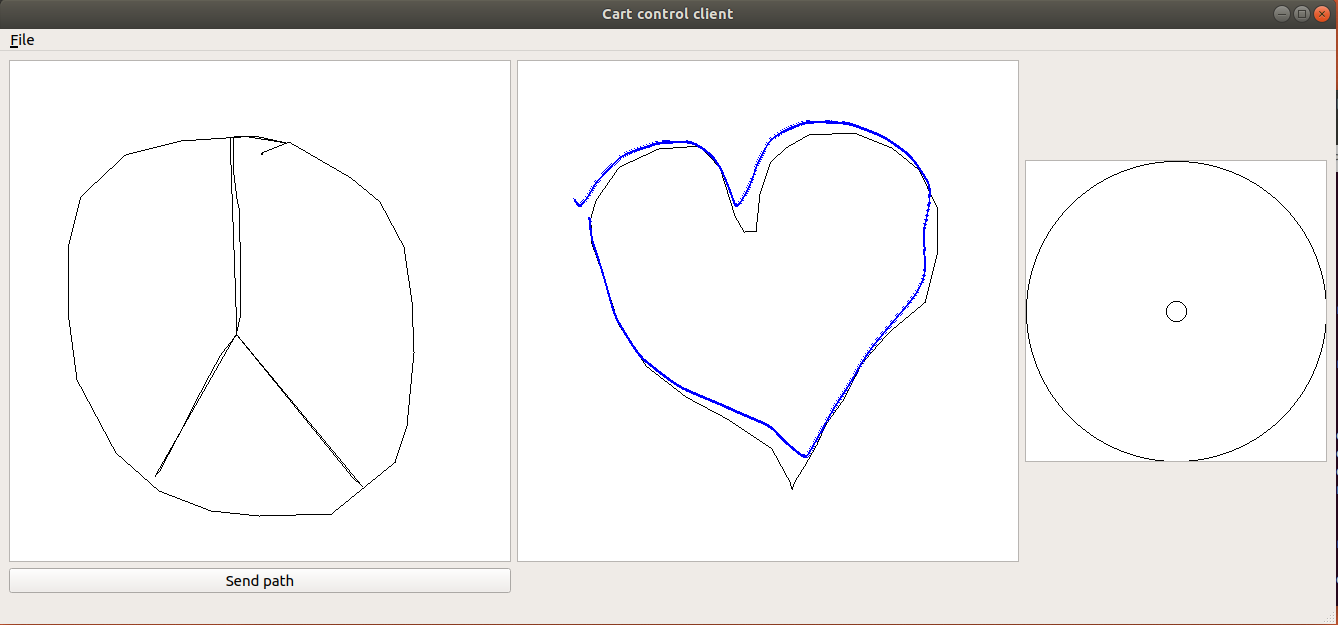
\includegraphics[width=\linewidth]{\picPath/Client/clinet.png}
\end{center}
  \caption{ Графический интерфейс клиента управления тележкой }
  \label{Figure:client}
\end{figure}

Программа состоит из трех виджетов, изображенных на рисунке \ref{Figure:client}. Слева-направо: виджет задания аналитического пути, виджет отображения положения робота и последнего пройденного аналитического пути, джойстик непрерывного управления скоростью тележки.   

Виджет задания аналитического пути описывается в файле cartpathsetter.h. 
Задание аналитического пути производится путем рисования ломаной линии на холсте. Границы координат, которые способен отобразить этот виджет -  от $-5$ до $5$ единиц по каждой из осей, поэтому путь задается только в этих пределах стимулируемой сцены. По нажатию кнопки, расположенной под виджетом, аналитический путь преобразуется в вектор точек и передается плагину управления путем передачи
сообщения по адресу темы /"имя_робота"/path. 
\iffalse
запроса, реализация которого описана в файле server.h. 
\fi
Кроме того, путь передается напрямую виджету отображения пути для его отрисовки. Клик правой кнопкой мыши позволяет отчистить холст виджета без отправки пути в плагин.

Виджет отображения пути описывается в файле cartpathgetter.h. Во время работы плагин публикует собственную позицию на плоскости в тему /"имя робота"/pos.  Эти данные читаются клиентским приложением посредством класса RosSubscriber, описанного в файле rospublisher.h. Средствами связи, встроенными в QT (технология сигналов и слотов), эти данные передаются виджету отображения положения робота. После публикации нового аналитического пути виджет удаляет уже отрисованные элементы и рисует аналитический путь. Границы координат, которые способен отобразить этот виджет - от $-5$ до $5$ единиц по каждой из осей. 

Виджет джойстика описывается в файле cartcontrollerwidget.h
Виджет получает координаты клика, вычисляет направление вектора скорости как разность между текущей координатой и серединой окружности джойстика  и вычисляет соответствующие скорости колес.  Функции преобразования вектора скорости тележки в скорости колес реализованны в файле cartkinematic.h и основываются на выводе главы \ref{chap:cartMovingAlg}. 
Класс этого виджета содержит в себе экземпляр издателя, класса RosPublisher, описанного в файле rospublisher.h.

 Класс RosPublisher с частотой 1000 герц публикует значение скорости, хранимое в поле velocity типа сообщения VelocityWheel,  описанного в файле /msg/VelocityWheel.msg. Для изменения публикуемой скорости в классе RosPublisher реальзовон метод setVelocity. Виджет джойстика вызывает метод setVeocity на последнем этапе передачи сообщения плагину, передавая преобразованную в угловые скорости колес глобальный вектор скорости.
 
  

\iffalse
\section{Моделирование управляемой голономной тележки}
\subsection{Определение движения тележки посредством плагинов Gazebo}
\section{Реализация управления моделируемой тележки}
\subsection{Управление тележкой посредством джостика}
\subsection{Реализация движения тележки по аналитически заданному пути}
\fi

\newpage
\addcontentsline{toc}{chapter}{Заключение}
\begin{center}
\bfseries ЗАКЛЮЧЕНИЕ
\end{center}

В результате работы были исследованы возможные типы передвижения робототехнических систем, в том числе распространенные виды колес. Изучена кинематика и динамика тележек, использующих $N$ омни-колес для передвижения, а также представлена кинематическая модель колеса меканума и четырехколесной тележки, использующей эти колеса. 

В системе ROS и  среде симуляции Gazebo разработана виртуальная модель трехколесного робота, использующего омни-колеса. Средствами ROS API и Gazebo API разработан плагин и клиент управления этим роботом. Разработан и успешно протестирован алгоритм передвижения робота по аналитически заданному пути, основанный на кинематической модели, разработанной в процессе дипломной работы.
\newpage
%список литературы
\addcontentsline{toc}{chapter}{Список использованных источников}
\begin{thebibliography}{0}

\bibitem{Siegwart}           	
Roland Siegwart
Introduction to Autonomous Mobile Robots /Roland Siegwart, Illah R. Nourbakhsh.
$-$ London, England
: The MIT Press, 2004. $-$ 321c.

\bibitem{MecanumWheel}
Klaus Zimmermann:
Dynamics of Mechanical Systems
with Mecanum Wheels / Klaus Zimmermann, Igor Zeidis, Mohamed Abdelrahman
$-$  Springer International Publishing Switzerland, 2014. $-$ 11с.

\bibitem{Ozhigov}
С. И. Ожегов.
Словарь русского языка
$-$ Мир и Образование, 2008. $-$ 1200с.

\bibitem{BigSovietEncycl}
Большая Советская Энциклопедия $-$ Советская энциклопедия, 1970.

\bibitem{WheelCmp}
Ksenia Shabalina.
Comparative Analysis of Mobile Robot Wheels
Design
/
Ksenia Shabalina, Artur Sagitov, Evgeni Magid.
$-$  Kazan, Russian Federation, Higher School of Information Technology and Information Systems
 2018. $-$ 5c.

\bibitem{SixLegsRobots}
Pavan Ramdya.
Climbing favours the tripod gait over alternative
faster insect gaits
/
Pavan Ramdya, Robin Thandiackal, Raphael Cherney, Thibault Asselborn1,Richard Benton ,
Auke Jan Ijspeert, Dario Floreano.
$-$ Nat. Commun 2017. $-$  11 с.

\bibitem{Saveliev}
И.В.Савельев.
Курс общей физики, том I.
Механика, колебания и волны, молекулярная физика.
$-$ Наука, 1970. $-$ 517c.

\bibitem{OmniWheelPatent}
US patent 1305535

\bibitem{OmniWheelPatentModern}
US patent 3789947

\bibitem{MecanumWheelPatent}
US patent 3876255

\bibitem{MecanumWheelCartDynamic}
А.А. Зобова.
Динамика экипажа с роликонесущими колесами
/ 
А.А. Зобова, Я.В. Татаринов. 
$-$ Прикладная математика и механика Том	73. Выпуск 1, 2009. $-$ 10 с.
\bibitem{ros.org}
Оффициальный сайт ROS. $-$ Текст: электронный. URL: https://www.ros.org/ (дата обращения: 25.10.2019 )

\bibitem{gazebosim.org}
Оффициальный сайт Gazebo. $-$ Текст: электронный. URL: http://gazebosim.org/ (дата обращения: 1.05.2020 )


\bibitem{pidBook}
Никулин Е.А. Основы теории автоматического управления. Частотные методы анализа и синтеза систем / учебное пособие $-$ БХВ-Петербург,2011. $-$ 632c.

\bibitem{RosBookTurtle}
YoonSeok Pyo.
ROS Robot Programming - First Edition
/
YoonSeok Pyo, HanCheol Cho, RyuWoon Jung, TaeHoon Lim
$-$  ROBOTIS Co.,Ltd, 2017. ISBN
 979-11-962307-1-5
 $-$ 460с.

\end{thebibliography}

\end{document}